%%%%%%%%%%%%%%%%%%%%%%%%%%%%%%%%%%%%%%%%%%%%%%%%%%%%%%%%%%%%
%%
%% LaTeX Thesis Template defined by Torsten Schön, May 2013
%%
%%%%%%%%%%%%%%%%%%%%%%%%%%%%%%%%%%%%%%%%%%%%%%%%%%%%%%%%%%%%
\documentclass[a4paper,11pt,twoside]{report}

% define marging document
\usepackage[a4paper,left=3cm,right=2cm,top=2cm,bottom=3cm,asymmetric]{geometry}

% define font arial
\usepackage{helvet}

\renewcommand{\familydefault}{\sfdefault}

% define spanish language
\usepackage[spanish]{babel}

\usepackage[utf8]{inputenc}

\usepackage[T1]{fontenc}

% import graphics
\usepackage{graphicx}

\graphicspath{{fig/}}

% custom month, year on Title
\usepackage{datetime}

\newdateformat{monthYear}{\monthname[\THEMONTH], \THEYEAR}

\makeatletter
\renewcommand{\monthnamespanish}[1][\month]{%
  \@orgargctr=#1\relax
  \ifcase\@orgargctr
    \PackageError{datetime}{Invalid Month number \the\@orgargctr}{%
      Month numbers should go from 1 to 12}%
    \or Enero%
    \or Febrero%
    \or Marzo%
    \or Abril%
    \or Mayo%
    \or Junio%
    \or Julio%
    \or Agosto%
    \or Septiembre%
    \or Octubre%
    \or Noviembre%
    \or Diciembre%
    \else \PackageError{datetime}{Invalid Month number \the\@orgargctr}{%
      Month numbers should go from 1 to 12}%
  \fi}
\makeatother

% caption into figure
\usepackage{caption}

\usepackage[font=small,skip=0pt]{caption}

% custom table
\usepackage{array} 

% space between bleeding
\setlength{\parindent}{0em}

% style for cite
\usepackage[autostyle]{csquotes}

% style bibliography
\usepackage{apacite}
\bibliographystyle{apacite}

% renew reference to bibliography
\renewcommand{\bibname}{Bibliografía}
\AtBeginDocument{\renewcommand{\bibname}{Bibliografía}}

% align text justify
\usepackage{ragged2e}

% degine source image
\newcommand{\source}[1]{\ttfamily #1}

% add code laguage programming
\usepackage{xcolor}
\usepackage{listings}

\lstset{
	%language = PHP, 
	commentstyle = \color{gray},
	extendedchars = \true,
	%inputencoding = utf8,
	keepspaces = true,
	keywordstyle = \bfseries,
	morekeywords = {function, return},
	numbers = left,
	captionpos = b,
	showspaces = false,
	showstringspaces = false,
	showtabs = false
}

% enumerate number item in list.
\usepackage{enumerate}

% define label caption listing
\renewcommand{\lstlistingname}{Segmento de Código}

% rename list of listing
\renewcommand{\lstlistlistingname}{Índice de segmento de códigos}

% landscape table
\usepackage{lscape}

% add appendix
\usepackage{appendix}

% add command about annes
\renewcommand{\appendixname}{Anexos}
\renewcommand{\appendixtocname}{Anexos}
\renewcommand{\appendixpagename}{Anexos}

% rename appendix to annex
\AtBeginDocument{\renewcommand\appendixname{Anexo}}

% enumerate table
\pagenumbering{roman}

% space after textquotedblright
\newcommand*{\textquotedouble}[1]{\textquotedblleft #1\textquotedblright}

% space bebind textgreater
\usepackage{xspace}

\let\OldTextGreater\textgreater

% vertical white space
\usepackage[compact]{titlesec}
    
\begin{document}

\newcounter{rom}


\begin{titlepage}
	
	\begin{tabular}[t]{l p{11cm} r}
	
\includegraphics[scale=0.6]{umss} & \centering \large{Universidad Mayor de San Simón} &	
\includegraphics[scale=0.7]{fcyt} \\
		& \centering \large{Facultad de Ciencias y Tecnología} & \\
		& \centering \large{Carrera Licenciatura en Ingeniería Informática} & \\
	\end{tabular}
	
	
	\begin{center}
		\normalsize
		
		\vspace{1.5cm}
		\Large{
		\textbf{Plataforma web educativa que gestione suscriptor de noticia para podcast producido por la Carrera de Lingüística Aplicada a la Enseñanza de Lenguas} 
		}		\\
	
		\vspace{1.5cm}
	
		\small
	\end{center}
		
	\begin{flushright}
	
		Proyecto de Adscripción para optar al \\ 
		Diploma Académico en Licenciatura \\ 
		en Ingeniería Informática	
		
	\end{flushright}
	
	\begin{center}
		
		\vspace{1.5cm}
			
		\textbf{Realizado por:} Juan Omar Huanca Balboa \\
	
		\vspace{1.5cm}
	
		\textbf{Tutor:} Mgr. Vladimir Costas Jauregui \\
		
		\vspace{1.5cm}
		
		Cochabamba - Bolivia
	
		\vspace{1.5cm}
					
		\monthYear\today
		
	\end{center}			

\end{titlepage}\thispagestyle{plain}
\cleardoublepage
\justifying
\noindent

%\chapter*{Dedicator\'{i}a}

Quiero dar mi agradecimiento a varias personas que formaron parte de este 
proyecto, desde su inicio proceso y conclusi\'{o}n. Dar gracias a Dios, 
luego tengo que dedicar este Proyecto de Adscripci\'{o}n en tres secciones:

Agradecer el apoyo incondicional a Mam\'{a} (Julia Balboa Choquecota) por su 
admirable ejemplo de responsabilidad, Pap\'{a} (Juan Huanca Bautista) por
su disciplina en el trabajo cotidiano, mil gracias por su ejemplo.

Agradesco el apoyo, sujerencias, observaciones, riesgos a consideras por mi 
tutor Mgr. Vladimir Costas Jauregui, gracias a su voto de confianza puesta en 
mi persona y por brindarme formar parte del equipo MEMI. Agradesco tambi\'{e}n
a Lic Marcelo Flores Soliz por sus observaciones en la elboraci\'{o}n del 
modelo conceptual, Ing. Jorge Orellana Araoz por brindar colaboraci\'{o}n en 
reformular mi perfil, Lic Rolando Jaldin Rosales por su colaboraci\'{o}n al 
momento de elaborar arquitectura de componentes y redacci\'{o}n de documentos. 
Ing. Claudia Ure\~{n}a por su apoyo moral.

Por terminar agradesco a mi colega de Trabajo Adscripci\'{o}n Rudy Rojas 
Gutierrez quien fue parte fundamental en el avance y mejoras sobre la Plataforma
, para los Adscritos de la Carrera Ling\"{u}\'{i}stica Aplicada a la 
Ense\~{n}anza de Lenguas (LAEL) al equipos de: Frances B\'{a}sico por sugerencias
en la mejorar de Actividades. Agradesco Lic. Manuel Camacho Arce como coordinador
del proyecto LAEL en la definici\'{o}n acertada en la nagevaci\'{o}n de 
interfaces, Mgr Rosario Saavedra Saravia por la iniciativa de implementar un 
proyecto entre las Carreras de Inform\'{a}tica y LAEL. 

\begin{flushright}
    Juan Omar Huanca Balboa
\end{flushright}\newpage\cleardoublepage
 
\tableofcontents
\listoffigures
\listoftables
\lstlistoflistings

%\chapter*{Ficha Resumen}

La creación de Recursos Multimedia Educativos son deseos provenientes de 
\'{a}reas como ser: Ciencias de la Educaci\'{o}n, Ling\"{u}\'{i}stica dentro la
UMSS.
De tal forma que coadyuven en fortalecer habilidades comunicativas que puedan 
llegar a tener la diversidad de personas en la sociedad.

A trav\'{e}s de Ley 269 promulgada 2 Agosto 2012, por el Presidente Evo Morales
en apoyo al fortalecimiento de idiomas dentro del Estado Plurinacional de 
Bolivia da a comprender que las lenguas originarias forman parte de la cultura,
la cultura es patrimonio del estado la cual la constitución debe de proteger a
pueblos reconocidos y personas hablantes.

En la gesti\'{o}n 2014 se realiza una convocatoria para un Proyecto de 
Adscripci\'{o}n, la cual enfoca los idiomas de Ingl\'{e}s B\'{a}sico, Frances
B\'{a}sico, Quechua B\'{a}sico, Quechua Psicosocial, Fon\'{e}tica Quechua, 
adem\'{a}s de contar con la colaboraci\'{o}n de Carreras de Inform\'{a}tica y
Sistemas. Considerado como un proyecto interdisciplinario como respuesta la
difusi\'{o}n de recursos por parte del \'{a}rea de Ling\"{u}\'{i}stica 
proponiendo para la sociedad como soluci\'{o}n parcial.

Se propone implementar un Servicio de Noticias basado en Podcast que son 
elaborados por propios Adscritos de Ling\"{u}\'{i}stica el mismo que este sujeto
a subscripci\'{o}n de noticias en la liberaci\'{o}n de Podcast en Audio/Video 
valga la redundancia brindando material educativo, gratuito para los funcionarios
p\'{u}blicos puedan descargar el Podcast y escucharlo en su tiempo libre para 
reforzar un conocimiento en el idioma Quechua formando un aprendizaje 
autorregulado.

En experiencia de trabajar con personas desarrollo y otras \'{a}rea de trabajo 
se recomienta manejar estandares de trabajo, adem\'{a}s de utilizar herramientas
open source para optimizar la elaboraci\'{o}n de recursos como ser: imagen, audio,
video, historietas debido que los mismos tendran que sujetarse estar a conexiones
lentas.\newpage\cleardoublepage

%\newpage
\thispagestyle{plain}~
\clearpage
\pagenumbering{arabic}

\chapter{INTRODUCCION}

\section{Introducción}

La Carrera de Lingüística Aplicada a la Enseñanza de Lenguas (LAEL) de la Universidad Mayor de
San Simon (UMSS) forma recursos a nivel personal acorde a su medio, proponiendo mecanismos para
la enseñanza y aprendizaje de lenguas. A mediados de la gestión 2013 se elaboró material 
educativo enfocado en habilidades comunicativas como ser: hablar, escribir, leer, pensar.
Haciendo hincapié en el auditivo por medio de recursos multimedia (Podcast) educativos 
a raíz de un análisis de necesidades a funcionarios públicos y/o privados de la urbe de
Cochabamba. Los estudiantes elaboraron recursos multimedia educativos enfocados en el 
aprendizaje autorregulado de la lengua Quechua.

Se propone proveer soporte tecnológico utilizando la difusión de canales de noticias de
Podcast basados en la liberación de cada Contenido (Episodio) para el usuario 
cibernauta pueda estar actualizado sobre el Programa de Aprendizaje, realizando una 
suscripción por lengua de interés.Con apoyo de las Tecnologías de la Información y
Comunicación enfocado en la enseñanza se pretende apoyar el proceso de Aprendizaje
Autorregulado de una lengua.

\section{Antecedentes}

Cualquier sitio Web es un espacio de información integrado. En muchos casos, sin embargo, este
espacio de información está de archivos HTML. Nos referimos a la ``arquitectura'' de la información
en lugar de la ``estructura'' o ``organización'' de la información con el fin de hacer hincapié en el
hecho de la estructura da forma el análisis de los requisitos funcionales del entorno. Para los
ambientes de aprendizaje, los requisitos funcionales son numerosos y no se han estudiado todavía
sistemáticamente.

Una plataforma virtual flexible será aquella que permita adaptarse a las necesidades de los alumnos
y profesores (borrar, ocultar, adaptar las distintas herramientas que ofrece); intuitivo, si su 
interfaz es familiar y presenta una funcionalidad fácilmente reconocible y, por último, amigable,
si es fácil de utilizar y ofrecer una navegabilidad clara y homogénea en todas sus páginas.

Internet se ha convertido hoy en día en el principal medio para publicar y difundir recursos e 
información en general. Podemos encontrar infinidad de recursos e información relevante para el 
desarrollo del proceso de enseñanza- aprendizaje destinado al profesorado y al alumnado. Sin embargo,
en esta categoría solo incluimos aquellos recursos que no son susceptibles de modificación y/o
publicación por parte de los usuarios, ya sean profesores o alumnos, en tanto que estos recursos serán
incluidos en la categoría de herramientas para la colaboración en red. Estos recursos serían recursos
web hipertextuales, generalmente páginas web y recursos para la docencia diseñados con aplicaciones
específicas, y bases de datos simulaciones, portales educativos y/o plataformas específicas de acceso a
información educativa y webquests. 

El podcast es uno de los recursos multimedia que ofrece la tecnología de hoy en día. Además, es una 
manera interactiva de aprendizaje que motiva y facilita los procesos de enseñanza y aprendizaje de una
segunda lengua. Por un lado, en la elaboración de los podcast se combinan los formatos: el texto, la imagen
y el sonido. Por otro lado, el uso de unos recursos multimedia (podcast) en la educación debe ser acorde a
la necesidad del aprendizaje o bien a los que exija la población estudiantes. Así también, Stanley define
el podcast de la siguiente manera:El podcast es un recurso disponible en la Internet, utilizado para crear
grabaciones de audio y hacerlas públicas en la red, la página principal del podcast tiene apariencia y puede
funcionar, como un blog. Además de los archivos de audio, se pueden agregar imágenes y comentarios. Los 
archivos de audio, una vez en la red, pueden funcionar como “radio” y ser descargados a computadoras 
personales, así como a CD o aparatos portátiles (MP3 o MP4) y ser escuchados tantas veces como sea de interés
del oyente en el sitio y hora de su conveniencia. Puede ser aplicado para cualquier
idioma

En general, los estudiantes se pueden describirse como autorregulado al grado que son meta cognitiva, 
'motivacional', y participantes conductivamente activos de su propio proceso de aprendizaje. Estos estudiantes personalmente inician y dirigen sus propios esfuerzos para adquirir conocimiento y habilidades en lugar de
confiar en los profesores, padres, u otros agentes de instrucciones. Para calificar específicamente como 
autorregulado en mi cuenta, los estudiantes deben incluir el uso de determinadas estrategias para alcanzar
metas académicas sobre la base del auto eficacia de perfecciones. Esta definición asume la importancia de tres
elementos: estrategias estudiantes de autorregulación del aprendizaje, las percepciones de auto eficacia de
rendimiento, habilidad y compromiso para metas académicas. Estrategias de aprendizaje autorregulado son 
acciones y procesos dirigidos a la adquisición de información o habilidad que involucra a la agencia, el
propósito y las percepciones instrumentales por alumnos. Estos incluyen métodos tales como la organización y la
transformación de la información, la búsqueda de información y ensayando o utilizando ayudas memoria. 

Se describe trabajos similares como: 

La Carrera LAEL impulsó en la creación de material multimedia bajo un estudio de necesidad de funcionarios 
públicos y/o privados en tener comunicación con personas quechua hablantes que migraron para contar con
beneficios como ser: hospital, colegio, juzgado, mercado de abasto, servicio de identificación personal, 
contextos dentro el área urbana de la ciudad de Cochabamba como producto salió una tesis en el año 2013 
:“Elaboración y Producción de Podcast para el aprendizaje Autorregulado de la Lengua Quechua”.

\section{Definición del Problema}

Actualmente LAEL carecen de soporte en el área de Tecnologías de la Información y
Comunicación (TIC's) enfocado la enseñanza debido a que no tienen materias
curriculares, ya que la actualización es por cuenta propia.
En la Facultad de Humanidades se cuenta con el área de Unidad Técnica de
Información (UTI), la misma se encarga de funciones: Control de Inventario de
Activos Fijos, Mantenimiento Preventivo–Correctivo de Equipos de Computación u
otros dispositivos electrónicos, Servicio de Red, Soporte al Usuario (Microsoft
office), Brindar Servicio Web página Facultativa, Gestión de Kardex. En general se
ocupan de soporte administrativo.
Los diferentes materiales educativos producidos por los diferentes Estudiantes de
Lingüística se encuentran en estado analógico debido a su falta de un medio de
difusión, quiere decir que permanece en estantes, bibliotecas. Lo cual limita al acceso
para los usuarios para quienes se desarrolló, muchos de ellos desconocidos por la
sociedad.
Haciendo hincapié que la educación tradicional que por sus buenos resultados en la
formación de profesionales en el área de la enseñanza de lenguas

Algunos Docentes de LAEL debido a su carencia de tiempo o interés en el
conocimiento de nuevas herramientas las cuales logren apoyar en la Educación
Superior tradicional es tomando como marco de referencia más por sus buenos
resultados.

Por lo mencionado anteriormente se define el problema como:

Escasa difusión de \textbf{recursos multimedia educativos} producidos por la Carrera de
Lingüística Aplicada a la Enseñanza de Leguas dificulta el desarrollo del \textbf{aprendizaje
autorregulado de las lenguas}.

\section{Objetivos}

\subsection{Objetivo General}

Contribuir con el \textbf{servicio agregado de noticias de Podcast} al fortalecimiento
del \textbf{aprendizaje autorregulado de lenguas} mediante el desarrollo de una
Plataforma Web Educativa.

\subsection{Objetivo Especifico}

\begin{itemize}

\item Proveer personalización de servicio agregador de noticias por programa de
aprendizaje (sub-categoría)

\item Implementar mecanismos de transcripción de contenido

\item Proveer representación de micro formatos para transcripción de contenido

\item Facilitar pruebas de servicio agregador de noticias, reproducción de Audio,
reproducción de Video.

\end{itemize}

\section{Justificación}
Implementar un mecanismo que coadyuve en el proceso de aprendizaje de lenguas
para un aprendizaje autorregulado.

Se realizara el proyecto con beneficio a los cibernautas que puedan completar su
habilidad auditiva y visual por medio de los Podcast.

La implementación del proyecto será realizado con tecnologías libres debido que se
trata de un proyecto de Adscripción nombrando como Unidad Patrocinadora es una
Institución Publica abocada en la formación de profesionales en el área de la
enseñanza y aprendizaje de lenguas.

\section{Alcance}

Se tendrán las siguientes áreas vistas dentro del proyecto:

\begin{itemize}

\item Gestión Servicio Agregador de Noticias
\item Animación de Transcripción.
\item Gestión de Micro formatos
\item Reporte de Pruebas

\end{itemize}\newpage\cleardoublepage

\chapter{NOTICIAS PODCAST}

\section{\textquestiondown Que son los feed de noticias?}

El feed \footnote{feed: Suministrar informaci\'{o}n} pueden ser m\'{a}s que t\'{i}tulos y enlaces, esto permite a los usuarios 
obtengan las \'{u}ltimas actualizaciones del sitio a diferentes dispositivos enviados desde un sitio web.

Los feeds pueden ser cualquier cosa de pocos titulares y enlaces a historia a todo el contenido del sitio, despojados
de su trazado y con metadatos aplicados generosamente. Sindicaci\'{o}n de contenidos permite a los usuarios experimentar
un sitio en varios dispositivos y ser\'{a}n notificados de cambios a trav\'{e}s de una variable de servicios. Puede 
variar desde una simple lista de enlaces enviados desde un sitio a otro a los inicios de la Web Sem\'{a}ntica.\cite{hammersley2005developing}

RSS y Atom son XML formatos para mensajes y otra informaci\'{o}n que es actualizada frecuentemente.
Los documentos que son escritos en estos formatos son llamados newfeeds or feed.\cite{wittenbrink2005rss}

Se define RSS \footnote{RSS: Really Simple Syndication} como un formato basado en XML \footnote{XML:Extensible Markup Language: designado para almacenar y transportar datos} para compartir contenido del sitio web.

Si un sitio web quiere compartir y publicar parte de su contenido a otros sitios en el mismo tiempo, el editor puede crear un
documento RSS. Este documento se puede publicar en el sitio web y cualquier usuario puede leer y utlizar diferentes sitios al mismo
tiempo. \cite{zeki2004rss}

Se utiliza la tecnolog\'{i}a feed de noticias para tener al usuario a los \'{u}ltimos contenidos en la aplicaci\'{o}n web
y este pueda notificarle via correo electronico del mismo con el t\'{i}tulo, descripci\'{o}n y categor\'{i}a al que pertenece.

\section{Sintaxis: RSS como XML formato}

Para muchos desarrolladores \textquotedblleft XML\textquotedblright y \textquotedblleft RSS\textquotedblright son sinominos. Se utiliza ambas tecnolog\'{i}as para el intercambios de informaci\'{o}n
en la Web.

Muchos sitios web identifican sus fuentes de noticias a trav\'{e}s de un bot\'{o}n de color naranja marcado \textquotedblleft XML\textquotedblright. Para muchos usuarios, y tambi\'{e}n para muchos desarrolladores \textquotedblleft XML\textquotedblright  y \textquotedblleft RSS\textquotedblright son sin\'{o}nimos. De hecho, todas las versiones del formato RSS y Atom son XML aplicaciones. Desde XML en s\'{i} es un metalenguage para definir idiomas par el intercambio de informaci\'{o}n en la
Web, los formatos de fuentes son tambi\'{e}n a menudo se llama \textquotedblleft dialectos XML\textquotedblright  o \textquotedblleft XML vocabularios \textquotedblright. A la fecha, RSS es el vocabulario, 
excepto XML de mayor \'{e}xito para tal XHTML, la versi\'{o}n XML de HTML.\cite{wittenbrink2005rss}

Se identifica un icono de color naranja que contiene en su interior un circulo y dos lineas curvas de color blanco para conocer
que la aplcaci\'{o}n web cuenta con subscripci\'{o}n.

\section{RSS 0.90}

Con RSS es posible integrar t\'{i}tulos desde otros sitios en la portada. Los usuarios deberian personalizar y suscribirse 
a un n\'{u}mero de canales que ofrece un canal de noticias RSS.


RSS fue inicialmente una abreviatura de \textquotedblleft RDF Site Summary \textquotedblright (Para obtener informaci\'{o}n acerca de RSS como
\textquotedblleft RDF Site Summary\textquotedblright consulte el Cap\'{i}tulo 3, Para una explicaci\'{o}n detallada del t\'{e}rmino, ver secci\'{o}n
3.1 RDF Fundamentos). Con RSS, es posible integrar los titulares de otros sitios con enlaces a estos sitios en el 
portal. El usuario puede personalizar el portal y suscribirse a un n\'{u}mero de sitios que ofrecen datos RSS.
De esta manera, My Netscape ten\'{i}a a su disposici\'{o}n una gran cantidad de contenidos adicional, que mantiene
a los usuarios en el sitio ya; los proveedores de datos RSS recibida tr\'{a}fico en el objetivo adicional m\'{a}s
importante de muchos sitios web en los tiempos de la boom de las punto-com. Puesta que es f\'{a}cil de convertir 
RSS a HTML. otros sitios pronto empezaron a utilizar la misma tecnolog\'{i}a. Slashdot pronto utiliza RSS en lugar
de su propio formato de t\'{i}tulo, y herramientas fueron desarrolladas para crear y el proceso de RSS en los 
lenguages de programaci\'{o}n comunes.\cite{wittenbrink2005rss}


Se tiene una tecnolog\'{i}a RSS, de tal forma que pueda obtener informaci\'{o}n de otros sitios en beneficio de
tener un lector de acceder a las noticias y no necesariamente acceder al sitio web.

\section{Los elementos de RSS 0.91}

Un importante version de Netscape RSS 0.91 a comparaci\'{o}n de RSS 0.90 de validar documentos de este formato
a comparacion de un DTD \footnote{DTD: Es un tipo de documento: define la estructura y legal elementos y atributos de un documento
XML}. 

La definitiva fuente de informaci\'{o}n respecto RSS 0.91 es la especificación de esta misma, pero para su 
conveniencias nosotros tenemos un diagrama Fig 2.1. Cada caja en el diagrama representa un elemento XML, 
y una fila indica contenci\'{o}n.\cite{johnson2006rss}

En la Figura 2.1, se tiene como composici\'{o}n de un feed que comprende la informaci\'{o}n de un canal de noticias y los elementos
que lo componenen, como categor\'{i}a primera se tiene la etiqueta <rss> seguido de <channel> a continuaci\'{o}n la informaci\'{o}n 
propia del canal de noticias: <title>, <link> y <description>. Tomando en cuenta los elementos se puede apreciar como segunda 
categoria a <item> que contiene: <title>, <link>y <description>.   

\begin{minipage}{1.0\textwidth}
	\centering
	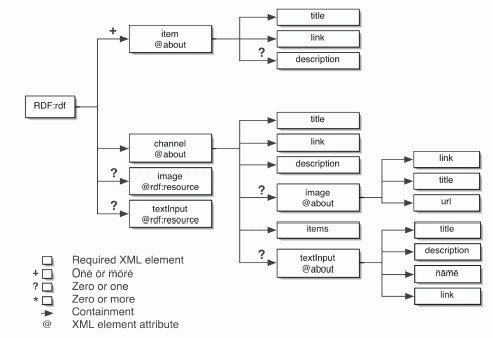
\includegraphics[scale=0.8]{rss091}
	\captionof{figure}{Elementos que componen un canal de noticias RSS 0.91.}
	\source{fuente: \cite{johnson2006rss}}

\end{minipage}


\section{RSS 1.0}

Un importante desarrollador Rael Dornfest quiso expandir el alcande de RSS. Por lo tanto ellos introducen
RDF \footnote{RDF :Resource Description Framework Schema un set de clases con ciertas propiedades.} y tambi\'{e}n un nuevo mecanismo, espacio de trabajo XML.

Otros desarrolladores importantes, sin embargo, entre ellos Rael Dornfest, que trabajaba como director de
tecnolog\'{i}a de O'Reilly, quer\'{i}a ampliar el alcance de RSS utilizando para otro prop\'{o}sitos y lo
conectan con formatos adicionales. Por lo tanto, se reintrodujeron RDF y tambi\'{e}n introdujo un nuevo
mecanismo, el espacio de nombres XML. Una especificaci\'{o}n relacionado fue publicado en diciembre de 2002;
los desarrolladores llaman el formato que se describe, RSS 1.0.\cite{johnson2006rss}

Esta norma, lanzado en diciembre de 2000, trajo dos cambios importantes en el mundo RSS: la introducci\'{o}n
de RDF y con ella una introducci\'{o}n de espacios de nombres.\cite{hammersley2005developing}
 
\subsection{Los elementos de RSS 1.0}

Comparando los RSS 0.91 y RSS 1.0 diagramas, tu puedes ver los formatos son significativos diferentes.
Aqui son las palabras diferentes:

\begin{itemize}

\item Un típico flujo RS 1.0 es más largo y más complejo, pero no lo hace incluir tantos metadatos como el
equivalente RSS 0.91 newfeed.

\item RSS 1.0 es más complejo, pero sólo porque es más flexible y extensible.

\item El elemento raíz es <RDF:rdf> en lugar de <rss>.

\item Las noticias existen como hijos de elemento raíz del documento y no como hijos del elemento <channel>,
como lo hacen en RSS 0.91.

\item Las noticias deben ser declaradas dentro del <channel> como recursos DRF. \par

En la Figura 2.2, para la composici\'{o}n de un feed se tiene como primera categor\'{i}a la informaci\'{o}n sobre el 
canal de noticias y como segunda categor\'{i}a la informaci\'{o}n sobre los elementos. En la primera  categor\'{i}a
se observa un documento RDF seguido de <channel> la cual se compone de: <title>, <link> y <description>. Como segunda
categor\'{i}a se tiene a <item> que se tiene especificado con un rdf:about el cual compone de: <title> , <link> lleva
un permamente enlace y <description>. 

\begin{minipage}{1.0\linewidth}
	\centering
	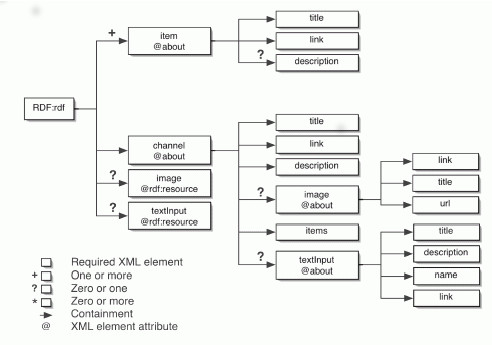
\includegraphics[scale=0.8]{rss010}
		\captionof{figure}{Los elementos XML que componen RSS 1.0}
		\source{fuente: \cite{johnson2006rss}}
\end{minipage}

\item <image> y <textinput> elementos deberian ser declarado dentro los <RDF:rdf> elementos son RDF
si han de ser incluidos dentro de la <channel> elemento.

\item Muchos elementos de metadatos, tales como  <pubDate>, <lastBuild-Time>, <skipDays>,
<skipHours>, <managingEditor>, y <webMaster> faltan del para. Estos se pueden añadir según sea necesario
mediante el uso de RSS 1.0 módulos, que se describen en la siguiente sección.\cite{johnson2006rss}

\end{itemize}

\section{RSS 2.0}

Se tiene RSS 2.0 esencialmente define sintaxis, El soporte de RSS 2.0 es considerado de baja especificaci\'{o}n
ya que es uno de los formatos de mayores ventajas.

Hoy en d\'{i}a, es el formato RSS feed m\'{a}s utilizado. Es caracter\'{i}stico de este formato no especifique,
o para dejar a los desarrolladores de aplicaciones para especificar: las conexiones entre Datos RSS, por una 
parte, entre otros formatos de contenido, datos/formatos de metadatos, y entornos de publicaci\'{o}n.\cite{wittenbrink2005rss}

\subsection{Los elementos de RSS 2.0}

\'{U}ltimamente RSS es ampliamente el formato m\'{a} usado. las conexiones entre RSS datos, contenidos de datos
en formatos/metadatos en otros entornos.

Hoy en d\'{i}a, es el formato RSS m\'{a}s utilizado. Es caracter\'{i}stico de este formato no especifique,
o para dejar a los desarrolladores de aplicaciones para especificar: las conexiones entre Datos RSS, por una
parte, entre otros formatos de contenido, datos/formatos de metadatos, y entornos de publicaci\'{o}n, por otro
lado. Esencialmente, RSS 2.0 define la sintaxis, en tanto que significado y el uso de determinaron mediante el
uso de ejemplos. Los partidiarios de RSS 2.0 consideran este bajo nivel de especificaci\'{o}n de una de las
mayores ventajas del formato, mientras que los partidiarios de las versiones de RSS alternas ven como su mejor
momento de debilidad.\cite{wittenbrink2005rss}

Esto, en realidad es la clave para el \'{e}xito de la RSS 2.0. La cosa m\'{a}s simple hay que hacer para hacer la validaci\'{o}n
de alimentaci\'{o}n es muy sencillo de hecho (vease el ejemplo 4.2). Si bien esto no es ninguna ayuda cuando usted est\'{a}
tratando de transmitir informaci\'{o}n compleja, como con RSS 1.0 o si usted est\'{a} tratando de construir un sistema centrada
en el documento completo, al igual que con Atom, es muy \'{u}til para muchas otras aplicacion.\cite{hammersley2005developing}

Los RSS 2.0 especificación provee una detallada descripci\'{o}n de cada elemento permitido en un RSS 2.0
newfeed. Tu puedes encontrar la especificaci\'{o}n aqu\'{i}  http://blogs.law.harvard.edu/tech/rss. Resumiendo
el XML que componen RSS 2.0, usando la misma notaci\'{o}n como nuestra previa figura, con un toque.\cite{johnson2006rss}

Se tiene un nueva version la cual conlleva las ventajas de las anteriores versiones y esta pueda ser manipulable por
lectores en equipos como agregadores online, tambien implementadas en applicaciones web.

En la Figura 2.3, Se tiene el primera categor'{i}a se tiene informaci'{o}n respecto al canal de noticias y como segunda
categor'{i}a los elementos de noticias que lo componen. Se habla sobre un canal de noticias conformado por lo siguientes
componentes: <title>, <link> y <description> requeridos. se tiene como elemento la etiqueta <item> comformado por los
componenetes <title> y <description> minimamente un ejemplar.

\begin{minipage}{1.0\linewidth}
	\centering
	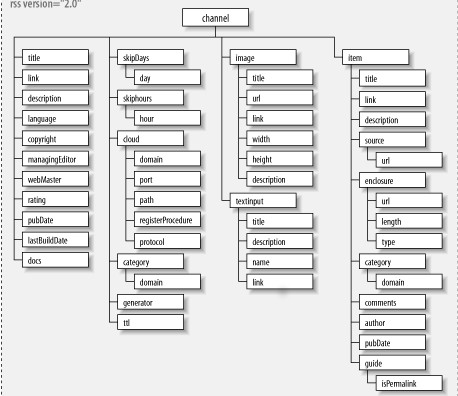
\includegraphics[scale=0.8]{rss020}
		\captionof{figure}{Los elementos XML que componen RSS 2.0}
		\source{fuente: \cite{johnson2006rss}}
\end{minipage}

\subsection{Plataforma Educativa LAEL}

En la Figura 2.4. Se tiene la realizaci\'{o}n de la subscripci\'{o}n de un canal de noticias, para ello el usuario deber\'{i}a
de encontrarse autentificado. 

\begin{minipage}{1.0\linewidth}
\centering
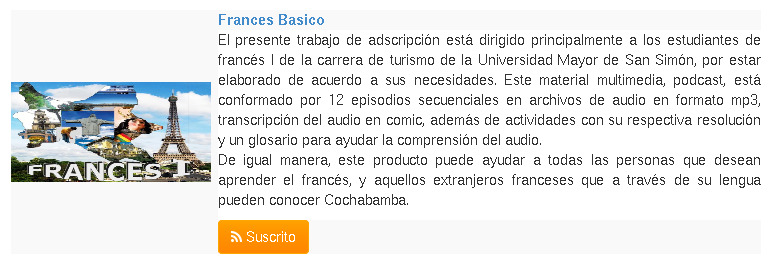
\includegraphics[scale=0.5]{basicFranceSubscribed}
\captionof{figure}{Subscripci\'{o}n Programa Aprendizaje Frances B\'{a}sico}
\source{fuente: (Elaboraci\'{o}n Propia)}
\end{minipage}

En la Figura 2.5. Se tiene uso de un navegador como Firefox, se puede utilizar un lector de noticias que encuentra disponible
y poder identifcar los diferentes elementos que contiene un feed de noticas: T\'{i}tulo, Fecha Liberaci\'{o}n
y Descripti\'{o}n.
 
\begin{minipage}{1.0\linewidth}
\centering
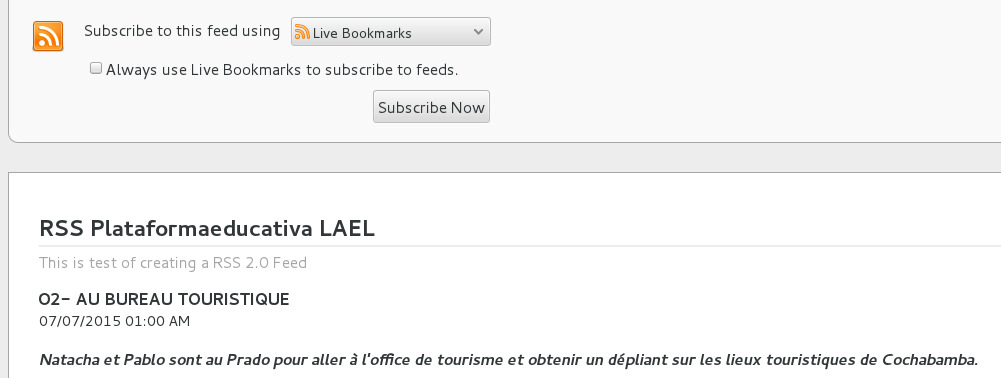
\includegraphics[scale=0.4]{basicFranceRssFirefox}
\captionof{figure}{Episodio1: Elemento canal de noticias}
\source{fuente: (Elaboraci\'{o}n Propia)}
\end{minipage}


\subsection{Las nueve versiones incompatibles de RSS}

Un influente blogger nombre Mark Pilgrim tiene que ser seguidor el desarrollador RSS de cerca, y el tiene que hacer
algunas importantes contribuciones. Trabajando con Sam Ruby, otro influente blogger, Pilgrim desarrollo servicio validacion de noticias lugar http://www.feedvalidator.org/ que maneja toda la comúnmente uso de RSS y Atom noticas
formato. 
Pilgrim señalaron que había nueve incompatibilidades versiones de RSS. Resumiendo estas incompatibles versiones y
autores, fecha y estado de cada una.\cite{johnson2006rss}

\begin{minipage}[b]{\hsize}\centering

\begin{tabular}{>{\centering\arraybackslash}m{.05\linewidth} |>{\centering\arraybackslash}m{.17\linewidth}|>{\centering\arraybackslash}m{.1\linewidth}|>{\centering\arraybackslash}m{.2\linewidth}|>{\centering\arraybackslash}m{.4\linewidth}}

& \textbf{Liberado por} & \textbf{Fecha} & \textbf{Estado} & \textbf{Nota} \\
\hline

\textbf{RSS 0.90} & Libby/Netscape & Enero 1999 & \textbf{Obsoleto} y rara vez se encuentra en la naturaleza & RDF- basado formato. \\
\hline

\textbf{RSS 0.91 } & Libby/Netscape & Julio 1999 & \textbf{Obsoleto} pero ampliamente usado & XML-basado con DTD; caído todos los elementos RDF; Añadido soporte para módulos. \\
\hline 

\textbf{RSS 0.91 (UserLand) } & Winer/Userland & Junio 2000 & \textbf{Obsoleto} pero ampliamente usado & caído DTD. \\
\hline 

\textbf{RSS 1.0} & RSS-DEV & Diciembre 2000 & \textbf{Viable} y ampliamente usado & RDF-basado formato nuevamente.\\
\hline

\textbf{RSS 0.92} & Winner/Userland & Diciembre 2000 & \textbf{Obsoleto} pero ampliamente usado & Contenido tipo de <description> elemento cambiado desde texto plano\\
\hline

\textbf{RSS 0.93} & Winer/Userland & Abril 2001 & \textbf{Obsoleto} y rara vez que se encuentra en la naturaleza & Aniadidp <pubDate> y <expirationDate> elementos. tambien permite multiples <enclousure> elementos por <item> \\
\hline

\textbf{RSS 0.94} & Winer/Userland & Verano 2002 & \textbf{Obsoleto} y rara vez que se encuentra en la naturaleza & eliminado <expirationDate> elemento. Especificación ya no está disponible en línea\\
\hline

\textbf{RSS 2.0} & Winer/Userland & Agosto 2002 & \textbf{Viable} y ampliamente usado. Final version de RSS & Permite adición de nuevos elementos siempre y cuando se definen por Espacio de nombres XML\\
\hline 

\textbf{RSS 2.0.1} & Winer/Harvard & Julio 2003 & Menor cambio a RSS 2.0 & Agregado elemento <rating>\\
\hline 

\end{tabular}

\captionof{table}{Las nueve versiones incompatibles de RSS}
\source{fuente: \cite{johnson2006rss}}
\end{minipage}

\section{El nuevo estandar: Atom}

A principios del 2003 un grupo de blooggers desilucionados con estado de newfeeds publicaron un nuevo estandar API
\footnote{API: Es un conjunto particular de reglas y especificaci\'{o}n que el programas pueden seguir para comunicarse entre si} el cual deberia ser conocido como Atom.

Atom es un formato de documento basado en XML que describe las listas de informaci\'{o}n relacionada conocida como
\textquotedblleft feeds\textquotedblright. Feeds se componen de una serie de elementos, conocidos como \textquotedblleft 
entradas \textquotedblright, cada uno con un conjunto extensible de metadatos adjunto.\cite{nottingham2005atom}

Si piensas Atom es una mejora sobre RSS o solamente otro formato, como un aplicación de blog usted 
tendra que aprender Atom. Todo el mayor servidor blog si soporta Atom ahora o tiene planes para hacer, y Blogger.com,
uno de los largos servicios blogging, ofrece solo Atom noticias - no RSS.\cite{johnson2006rss}


\subsection{Los elementos de Atom}


Nosotros tenemos usado la notación <text>, <person>, y <fecha> a indicar cuales elementos son constructores
comunes. Requeridos elementos son compartidos.

En la Figura 2.6, se tiene como primera categor\'{i}a al <feed> como cananl de noticas y sus datos de informaci\'{o}n,
como segunda categor\'{i}a se tiene los componentes que tiene un <entry>. La primera categor\'{i}a comprende un 
<title>, <link>, <link> con la propiedad rel="self", <update> y <autor>. En la segunda categor\'{i}a el elemento <entry>
esta compuesto por: <title>, <link>, <id>, <published> y <update> ademas de contener una subcategor\'{i}a denominada
la etiqueta <content> con la propiedad type="xhtml".

\begin{figure}[!ht]
\centering
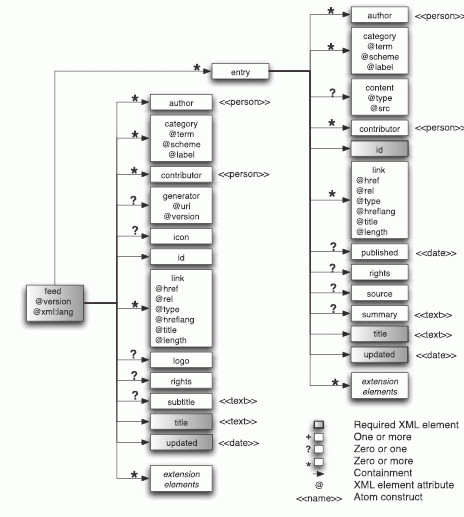
\includegraphics[scale=0.8]{elementsXML}
\caption{Los elementos XML que conforman un servicio de noticias Atom}
\source{fuente: \cite{johnson2006rss}}
\end{figure}


Algunos requisitos importantes no son evidentes a partir de este diagrama formato Atom, Por lo tanto permiteme
revisar ellos. Primero, el nivel feed requisito.

\begin{itemize}

\item El feed debe contener un <id> elemento.
\item El feed debe contener un <link> con rel="self" que contiene un enlace to el feed mismo. Esto hace posible para
un programa, cual puede tener solo una copia de un documento de noticias, a encontrar la URL de las noticias.
\item El feed debe incluir un solo enlace, significando un <link> elemento con rel="alternate" - tipicamente un enlace
alternativo de un alimento hace referencia a una alternativa representación de la alimentación.
\item El autor debe ser especifico lugar el nivel feed o en cada individual entrada.

\end{itemize}

Y ahora, en cada nivel requiere.

\begin{itemize}

\item Cada entrada debe contener un <id> elemento.
\item Si la entrada no tienen un <content> elemento, deberia tener una alternativo enlace. Un enlace alternativo es su enalce
permanente, un enlace permanente entradas representacion web.
\item Un enlace puede tener multiples enlaces alternativos para diferentes lenguajes y tipos de contenidos, pero una entrada
deberia no contener mas que una enlace alternativo para cada combinacion de languages y tipo de contenido.
\item La entrada deberia incluir un <summary> elemento si el contenido es no facilmente leible, por ejemplo es no <content> 
elemento, el <content> elemento contiene algun otro texto, o el <content> referencia de elementos contenido en otros lugares.\cite{johnson2006rss}

\end{itemize}

\subsection{Podcasting con Atom}


Podcasting originado como una caracteristica de RSS, pero a medida que el mundo se mueve Atom como el nuevo estándar.
Los podcasters también lo hará - y para buenas razones. Atom puede soportar podcasting a travez del elemento <link>.
Como es el caso con RSS 2.0-basado podcasts, usted puedes tener solo un podcast por entrada. Pero con Atom, tu puedes
tener diferentes representacion por cada lenguage y por cada tipo de contenido.\cite{johnson2006rss}

La Figura 2.7, Se tiene la evoluci\'{o}n y los distintos caminos tomados por los formatos por RSS y Atom en transcurir del
tiempo

\begin{figure}[!htb]
\centering
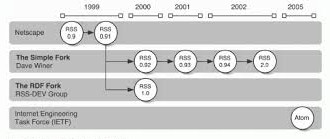
\includegraphics[scale=1]{newsFeed}
\caption{News feed árbol formato}
\source{fuente: \cite{johnson2006rss}}
\end{figure}
\newpage\cleardoublepage

\chapter{HERRAMIENTAS DE DESARROLLO}

\section{TICs en la Educaci\'{o}n}

Es importante entender que las TICs \footnote{TICS: Tecnolog\'{i}as de la 
Informaci\'{o}n y de Comunicaci\'{o}n \cite{severin2013enfoques}} no son s\'{o}lo herramientas, uno de ellos
se tiene cuando la persona queda excluida del acceso y uso de las TICs es como si
estubiera dejando de interactuar con el mundo exterior, incluso se habla de que 
el acceso tecnolog\'{i}a y conectividad como un derecho hacia un bien b\'{a}sico.

El primer foco de la atenci\'{o}n definido es el considerar la manera en que las TICs
favorecen el desarrollo de nuevas pr\'{a}cticas educativas, m\'{a}s pertinenetes y eficaces,
lo que incluye fortalecer el protagonismo que tienen los docentes en los cambios
educativos.\cite{severin2013enfoques}

\section{Educaci\'{o}n y virtualidad: hacia un espacio de vivencia de valores}

La relaci\'{o}n entre la educaci\'{o}n y la virtualidad es de creatividad. La 
educaci\'{o}n a trav\'{e}s de la web explica las did\'{a}ctivas de cualquier 
acci\'{o}n educativa. 

Educaci\'{o}n y virtualidad se complementan para que la educaci\'{o}n pueda 
disfrutar de las posibilidades creativas de la virtualidad con la mejora de sus
procesos y las acciones encaminadas a la ense\~{n}anza y al aprendizaje, mientras
que la virtualidad se beneficia de la metodolog\'{i}a necesaria en algunos casos,
como cuando la finalidad sobrepasa la mera informaci\'{o}n.
\cite{duart2000aprender}

\section{Web 2.0}

Sin embargo, algunas de las caracter\'{i}sticas t\'{i}picas asociadas con los sitios
Web 2.0 las siguientes:

\begin{itemize}

\item \textbf{El uso compatible con los est\'{a}ndares HTML y CSS} Esto permite a
 los sitios de trabajo a trav\'{e}s de muchas plataformas, formas y ayuda con la
 accesibilidad.
\item \textbf{El Uso de Ajax para proveer una interfaz usuario rica} Mediante la
realizaci\'{o}n operaciones triviales de fondo usando XMLHttpRequest 
\footnote{XMLHttpRequest: Define una API que proporciona un gui\'{o}n 
funcionalidad de cliente para transferir datos entre un cliente y un servidor 
\cite{xmlHttpRequest}} , p\'{a}ginas web pueden ser m\'{a}s funcional e 
intuituva.
\item \textbf{Compartiendo datos mediante Web feeds y servicios web} Los
usuarios les gusta agregar muchos feeds a recibir f\'{a}cilmente actualizaci\'{o}nes
de contenido de sus sitios favoritos con v\'{i}nculos Web.
\item \textbf{La Incorporaci\'{o}n de herramientas en redes sociales} Blogs y foros 
puede permitir a los usuarios comunicarse entre s\'{i}.
	
\end{itemize}

Aunque ninguna de estas caracter\'{i}sticas o aspectos del desarrollo son nuevos,
utilizamos la Web 2.0 t\'{e}rmino para describir la actual generaci\'{o}n de sitios
web que hacen un buen uso de HTML y CSS, mientras que tal vez mejorar su interfaz
con el Ajax y herramientas de redes sociales.\cite{zervaas2007practical}

\section{Arquitectura Cliente/Servidor}

Arquitecturas cliente-servidor son generalmente consideradas como arquitecturas
de sistemas distribuidos, pero el modelo l\'{o}gico de servicios independientes
que se ejecutan en servidores separados puede implementarse en un solo equipo.
Una vez m\'{a}s, un beneficio importante es la separaci\'{o}n e independencia.
Los servicios y servidores se pueden cambiar sin afectar otras partes del sistema.

Los clientes pueden tener que saber los nombres de los servidores disponibles y
los servicios que ellos proveen. Sin embargo, los servidores no necesitan conocer
la identidad de los clientes o c\'{o}mo muchos clientes tienen acceso a sus
servicios. Los clientes acceden a los servicios prestados por un servidor a 
trav\'{e}s de llamadas a procedimientos remotos utilizando un protocolo de 
petici\'{o}n-respuesta como el http protocolo utilizando en la WWW, Esencialmente,
un cliente realiza una solicitud a un servidor y espera que reciba una respuesta.

Figura \ref{Una arquitectura cliente-sevidor para una filmoteca} es un ejemplo de
un sistema que se basa en el modelo cliente-servidor. Esta es un sistema basado en
la web multi-usuario para proporcionar una biblioteca de cine y  fotograf\'{i}a.
En este sistema, varios servidores de gesti\'{o}n, se muestran los diferentes tipos de
medios.\cite{sommerville2011software}

\begin{figure}[!htb]
	\centering
	\fbox{
		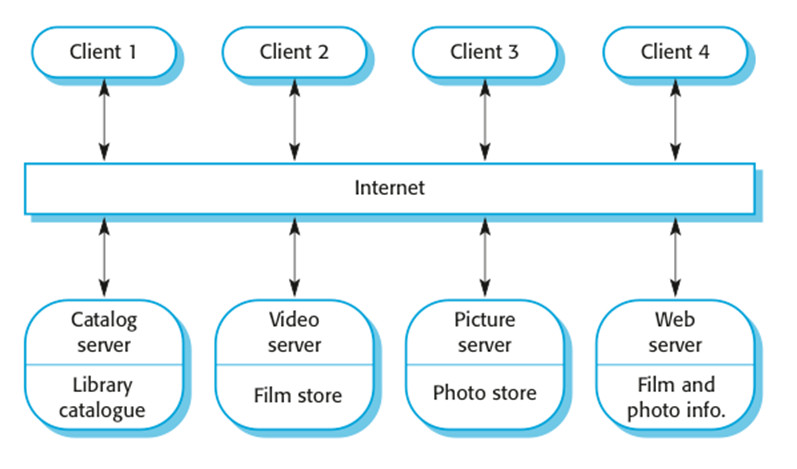
\includegraphics[scale=0.5]{architectureClientServer}
	}
	\caption{Una arquitectura cliente-sevidor para una filmoteca}
	\source{fuente: \cite{sommerville2011software}}
	\label{Una arquitectura cliente-sevidor para una filmoteca}
\end{figure}

\subsection{Patr\'{o}n Dise\~{n}o: Modelo Vista Controlador}

La idea de los patrones como una forma de presentar, compartir y reutilizar el
conocimiento sobre sistemas de software ahora se utiliza ampliamente.

Usted puede pensar en un patr\'{o}n arquitect\'{o}nico como una estilizada 
descripci\'{o}n, abstracta de buena pr\'{a}ctica, que ha sido probada en 
diferentes sistemas y entornos. Asi que, un patr\'{o}n arquitect\'{o}nico
debe describir una organizaci\'{o}n del sistema que ha sido con \'{e}xito
en los sitemas anteriores. Debe incluir informaci\'{o}n de cu\'{a}ndo es
y no es apropiado utilizar ese patr\'{o}n, y los patrones de puntos fuertes
y d\'{e}biles.

Figura \ref{Arquitectura de aplicaciones Web utilizando el patr\'{o}n MVC} muestra
una posible arquitectura de tiempo ejecuci\'{o}n cuando este patr\'{o}n se utiliza
para la gesti\'{o}n de la interacci\'{o}n en un sistema basado en la web.

En una secci\'{o}n corta de un cap\'{i}tulo general, es imposible describir todos
los patrones gen\'{e}ricos que se pueden utilizar en el desarrollo de software.
M\'{a}s bien, les presento algunos ejemlos seleccionados de los patrones que se
utilizan ampliamente y que la captura de los buenos principios de dise\~{n}o 
arquitect\'{o}nico. He incluido algunos ejemplos m\'{a}s de los patrones 
arquitect\'{o}nicos gen\'{e}ricos en las p\'{a}ginas web del libro.
\cite{sommerville2011software}

\begin{minipage}{1.0\textwidth}
	\centering
	\fbox{
		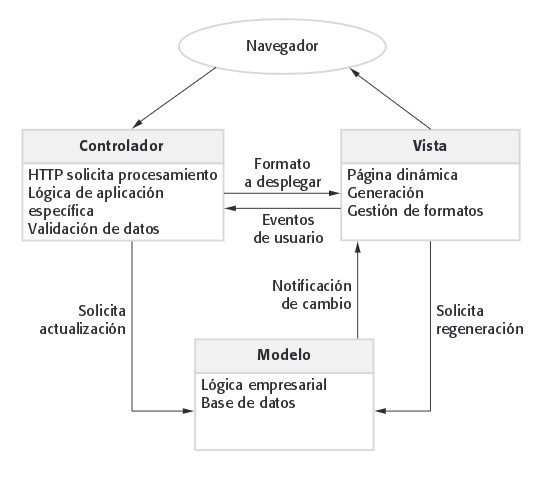
\includegraphics[scale=0.8]{mvcPattern}
	}
	\captionof{figure}{Arquitectura de aplicaciones Web utilizando el patr\'{o}n MVC}
	\source{fuente: \cite{sommerville2011software}}
	\label{Arquitectura de aplicaciones Web utilizando el patr\'{o}n MVC}
\end{minipage}

\begin{itemize}

\item \textbf{Dise\~{n}o del Proyecto}

Se toma como patr\'{o}n de Dise\~{n}o Modelo Vista Controlador como base para 
extender la funcionalidad de un Controlador denominado Manager la cual realiza
una abstracci\'{o}n de funcionalidad y reuso esta definido en la Figura 
\ref{Arquitectura Extendida MVCM}

\begin{minipage}{1.0\textwidth}
	\centering
	\fbox{
		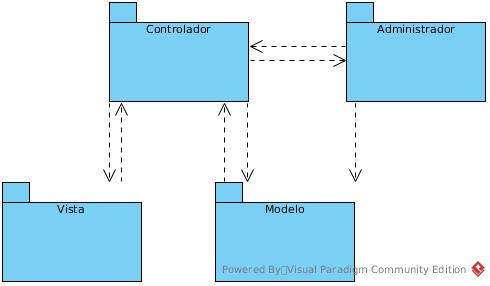
\includegraphics[scale=0.5]{mvcm}
	}
	\captionof{figure}{Arquitectura Extendida MVCM}
	\source{fuente: (Elaboraci\'{o}n Propia)}
	\label{Arquitectura Extendida MVCM}
\end{minipage}


\end{itemize}

\section{PHP}

PHP siempre ha sido un lenguaje que es especificamente \'{u}til para la 
programaci\'{o}n web. Eso sigue siendo, y con PHP5, se ha criado al d\'{i}a y
se estableci\'{o} un lenguaje que es totalmente compatible con los modernos 
m\'{e}todos orientados a objectos, pr\'{a}cticas y principios. 

Versi\'{o}n 5 de PHP \footnote{PHP: Hypertext Processor \cite{reiersol2007php}} 
es, cuanto otras cosas, un intento de hacer el uso de estos conceptos y 
metodol\'{o}gicas herramientas en PHP.\cite{reiersol2007php}

\subsection{Yii Framework}

Con Yii, los conceptos m\'{a}s importantes son Programaci\'{o}n orientada a objetos
(POO) y el patr\'{o}n Modelo-Vista-Controlador (MVC).

A diferencia de otros frameworks \footnote{framework: Es un conjunto de recursos
y herramientas para desarrolladores de software para crear y gestionar 
aplicaciones web, servicios web y sitios web. \cite{framework}} , Yii siempre ha
requerido la versi\'{o}n 5 de PHP. Esto significa, ya que PHP 5 tiene una 
estructura objeto sumamente mejorada y avanzada en comparaci\'{o}n con el 
mayores PHP 4. \cite{ullman2013yii}

\textbf{Extensiones Yii}

Se define extensiones como una abstracci\'{o}n de funcionalidad espec\'{i}fica, el
mismo puede ser utilizado en sistemas o applicaciones web: Envio de correo, 
autentificaci\'{o}n por red social, dise\~{n}o web responsivo, etc.

\begin{enumerate}

\item \textbf{Booster}

YiiBooster es una colecci\'{o}n de widgets \footnote{widgets: Es un elemento 
de una interfaz gr\'{a}fica de usuario que muestra informaci\'{o}n o 
proporciona una forma espec\'{i}fica para un usuario interactuar con el sistema
operativo o una aplicaci\'{o}n \cite{widget}} que faciliten la tarea de 
desarrollar aplicaciones Yii, as\'{i} como, dando a su aplicaci\'{o}n un poco 
de impulso. B\'{a}sicamente, Booster fuerza a los retos m\'{a}s comunes que los
desarolladores Yii enfrentan al tratar de mejorar sus aplicaciones. \cite{booster}

\item \textbf{CascadeDropDown}

Es simple de utilizar la extensi\'{o}n el plugin de JQuery JQuery-cascada para
rellenar los datos de una lista desplegable depende de un ajax/ getJSON-llamada.
 \cite{cascadedropdown}

\item \textbf{Efeed}

RSS Escritor Generador de extensi\'{o}n para crear tus feeds. Actualmente soporta
RSS 1.0, RSS 2.0 y ATOM 1.0. \cite{efeed}

\item \textbf{Hoauth}

Proveedor yii-oauth sencilla integraci\'{o}n con la red social, la autorizaci\'{o}n
lib Hybridauth \footnote{Hybridauth: Meta HybridAuth es actuar como un api 
abstracta entre la aplicaci\'{o}n y diversos apis sociales e identidades 
proveedores como Facebook, Trwiter y Google \cite{hybridauth}} en Yii. \cite{hoauth}

\item \textbf{Image}

Proporciona m\'{e}todos para la manipulaci\'{o}n din\'{a}mica de las im\'{a}genes.
Varios formatos de imagen como JPG, PNG, GIF y puede cambiar de tama\~{n}o, recortar,
rotar. \cite{image}

\item \textbf{MediaElement}

Esta extensi\'{o}n le permite agregar HTML5 reproductor de audio y v\'{i}deo 
utilizando la biblioteca MediaElementJS para su proyecto Yii. \cite{mediaelement}

\item \textbf{Yii-Image-Zoomer}

Es flexible, eficiente, m\'{a}s peque\~{n}o, tiene m\'{a}s funciones y m\'{a}s
robusta, la compatibiliadad entre navegadores. \cite{yiiImageZoomer}

\item \textbf{YiiMailer}

Extensi\'{o}n Yii para el env\'{i}o de mensajes de correo electr\'{o}nico HTML
con dise\~{n}os utilizando PHPMailer \footnote{PHPMailer: Es una de las 
bibliotecas de PHP de c\'{o}digo abierto m\'{a}s populares para enviar mensajes
de correo electr\'{o}nico \cite{phpMailer}} \cite{yiiMailer}

\end{enumerate}


\section{JavaScript} 

JavaScript es el lenguaje de programaci\'{o}n de la Web. La inmensa mayor\'{i}a
de la p\'{a}gina web moderna utiliza JavaScript y todos los modernos navegadores
web en ordenadores de sobremanera, consolas de juegos, mesas y tel\'{e}fonos 
inteligentes incluyen int\'{e}rpretes de JavaScript, haciendo JavaScript m\'{a}s
lenguaje de programaci\'{o}n  omnipresente en la historia. JavaScript es parte de
la tr\'{i}ada de tecnolog\'{i}as que todos los desarrolladores web deben aprender:
HTML para especificar el contenido de p\'{a}ginas web, CSS para especificar la 
presentaci\'{o}n de las p\'{a}ginas web y JavaScript para especificar el comportamiento
de las p\'{a}ginas web. \cite{flanagan2006javascript}

\subsection{JQuery}

JQuery es una biblioteca JavaScript de c\'{o}digo abierto que simplifica las 
interacciones entre un Documento HTML, o m\'{a}s precisamente el Documento 
Object Model (tambi\'{e}n conocido como el DOM), y JavaScript.

Espec\'{i}ficamente, JQuery simplifica documento HTML de desplazamiento y la 
manipulaci\'{o}n, manejo de eventos del navegador, animaciones DOM, interacciones
Ajax y cross-browser desarrollo JavaScript.\cite{lindley2009jquery}

\section{HTML5}

HTML fue dise\~{n}ado originalmente para, compartir est\'{a}tica documento basado
en texto en el Internet. Con el tiempo, ya que los usuarios de Internet y los 
dise\~{n}adores quer\'{i}an m\'{a}s interactividad en su documento HTML, comenzaron
a mejorar estos documentos, a\~{n}adiendo funcionalidad forma y capacidades tempranas
\textquotedblleft portal\textquotedblright tipo. Ahora, estas colecciones de 
documentos est\'{a}ticos, o de los sitios web, se aparecen m\'{a}s a las aplicaciones
web, basado en los principios del rico escritorio de aplicaciones cliente/servidor.
Estas aplicaciones web est\'{a}n siendo utilizadas en la mayor de dispositivos: 
ordenador, port\'{a}tiles, tel\'{e}fonos inteligentes, tabletas de la gama.

HTML5 hace que las aplicaciones web m\'{a}s usables, as\'{i}, ya que elimina la
necesidad para los plugins. \cite{wang2013definitive}


\section{CSS}

Los usuarios deben ser capaces de acceder a su contenido sin importar qu\'{e} 
dispositivo utilizan o qu\'{e} software est\'{a} en esos dispositivos. CSS 
permite a los desarrolladores de bien c\'{o}mo se ve el contenido, incluyendo 
m\'{e}todos para la costura o la presonalizaci\'{o}n de la presentaci\'{o}n del
contenido basado en el dispositivo. Por ejemplo, los usuarios pueden acceder a su
contenido a trav\'{e}s de un navegador en un netbook, un navegador en un t\'{e}lefono,
en su TV, con un lector de pantalla, como una presentaci\'{o}n, o incluso impreso
en formato PDF. CSS proporcina mecanismos de estafa arrastre la apariencia o 
presentaci\'{o}n de su contenido, no importa el dispositivo.\cite{weyl2012s}

\subsection{Bootstrap}

En los dias anteriores de Twitter, los ingenieros utilizan casi cualquier 
biblioteca que estaban familiarizados para satisfacer las necesidades de 
front-end. Las incoherencias entre las aplicaciones individuales hechas dif\'{i}ciles
de escalar y mantener ellos. Bootstrap comenz\'{o} como una respuesta a estos 
desaf\'{i}os y se aceler\'{o} r\'{a}pidamente durante la primera semana Hack de
Twitter. A finales de Hack semana tuvimos llegado a una versi\'{o}n estable que
los ingenieros podr\'{i}an utilizar en toda la compa\~{n}ia.\cite{spurlock2013bootstrap}

\subsection{CSS3}

Hasta el momento, el Grupo de Trabajo de CSS en el W3C ha comenzado a trabajar 
en m\'{a}s de 40 m\'{o}dulos de CSS. Agunos m\'{o}dulos, como selectores, 
espacios de nombres, Color y Medios de consultas, se considera estable y son ya
sea en Candidata a Recomendaci\'{o}n o el estado de recomendaci\'{o}n. El primer
m\'{o}dulo se convierta en una Recomendaci\'{o}n del W3C fue el CSS3 M\'{o}dulo
de color, publicado el mismo d\'{i}a que la especificaci\'{o}n CSS 2.1 se convirtio
en una recomendaci\'{o}n. El trabajo en diferentes m\'{o}dulo ha progresado a 
diferentes velocidades. Los bloqueos en un m\'{o}dulos ha progresado y se sostiene
cualquier otro m\'{o}dulo.\cite{spurlock2013bootstrap}

\section{Git}

El control de versiones es un sistema que registra cambios en un archivo o conjunto
de archivos con el tiempo para que pueda recuperar versiones especif\'{i}cas mas tarde.

Si usted es un dise\~{n}ador gr\'{a}fico o web y desea mantener todas las versiones
de una imagen o el dise\~{n}o (que usted sin duda que desee), un sistema de control
de versiones (VCS) es una cosa muy aconsejable utilizar. Te permite revertir los
archivos de nuevo a un estado anterior, revertir todo el proyecto de nuevo a un
estado anterior, comparar cambios en el tiempo, a ver qu\'{i}en dura modificado
algo que podr\'{i}a ser la causa de un problema, que se present\'{o} un problema
y cuando, y m\'{a}s.\cite{chacon2009pro}

\section{Pivotal Tracker}

Es una herramienta simple, basado en la historia de planificaci\'{o}n del proyecto
que permite a los equipos a colaborar y reaccionan instant\'{a}neamente a los 
cambios del mundo real. Se basa en m\'{e}todos de desarrollo de software \'{a}giles,
pero se puede utilizar en una variedad de tipos de proyectos. Rastreador te libera
para concentrarse en las cosas, sin empantanarse, manteniendo sus planes en 
sincron\'{i}a con la realidad. \cite{pivotalTracker}\newpage\cleardoublepage

\chapter{FORTALECIMIENTO DEL APRENDIZAJE AUTORREGULADO EN CARRERA LAEL}

\section{Objeto Formativo}

Formar profesionales para comprometerse con su medio con agente de cambio, 
interpretar la realidad educativa nacional, particularmente la ling\"{u}\'{i}sta,
proponiendo metodolog\'{i}as espec\'{i}ficas para la ense\~{n}anza de lenguas
extranjeras, del castellano y el quechua, lengua extranjera y/o segunda.

\section{Perfil Profesional del Estudiante en la Carrera LAEL}

El estudiante en la Carrera LAEL el documento denominado \textquotedblleft 
Correspondencia y recibida y Despachada\textquotedblright del a\~{n}o 2009,
destac\'{o} el Perfil profesional del Estudiante de la Carrera LAEL constituido
textualmente de la siguiente manera:

\begin{enumerate}

\item Un profesional comprometido con su medio en el que gracias a procesos de
investigaci\'{o}n de la realidad boliviana aplicara m\'{e}todos y t\'{e}cnicas
adecuados dentro del proceso de ense\~{n}anza aprendizaje de lenguas en el 
sistema educativo nacional y universitario
\item Ser capaz de evaluar y adaptar m\'{e}todos de ense\~{n}anza, tanto para
las lenguas extranjeras como para el castellano y el Quechua: lengua extranjera
y/o segunda lengua.
\item Realizar investigaci\'{o}n interdisciplinaria para estudios e 
interpretaci\'{o}n sobre:
	\begin{itemize}
	
	\item La ense\~{n}anza de lenguas en el sistema educativo
	\item Problemas de alfabetizaci\'{o}n en nuestro pa\'{i}s, aportando desde la
	perspectiva de las lenguas
	\item Problemas espec\'{i}ficos de biling\"{u}ismo y de las relaciones entre 
	la lengua materna y la segunda lengua.
	\item Caracter\'{i}stica del castellano boliviano en sus diferentes niveles
	culturales
	
	\end{itemize}
\item Investigar sobre las lenguas, realizando estudios comparativos de sistemas
de comunicaci\'{o}n y estructuras de las lenguas en todos los niveles de 
ense\~{n}anza
\item Evaluador de contenidos de las asignaturas relacionadas con el \'{a}rea de
lenguas en todos los niveles de ense\~{n}anza
\item Desempe\~{n}ar eficientemente en cualquier otro campo en el que exija 
conocimiento y formaci\'{o}n de lenguas (Documento Carrera Ling\"{u}istica 
Aplicada a la Ense\~{n}anza de lenguas 2009)

\end{enumerate}

El perfil profesional del estudiante de la Carrera Ling\"{u}istica Aplicada a la
Ense\~{n}anza de lenguas, se\~{n}ala que los objetivos est\'{a}n enfocados en su
mayor\'{i}a en el \'{a}rea de t\'{e}cnicas que corroboran al \'{a}mbito educativo
a trav\'{e}s de la ense\~{n}anza de las lenguas(L1 y L2).

Este documento a\'{u}n se mantiene en desarrollo y sin modificaci\'{o}n alguna.
\cite{Q2014}

\section{Objetivos Generales}

El licenciado en LAEL ser\'{a} capaz de:

\begin{itemize}

\item Desenvolverse en su medio como agente de cambio, comprometi\'{e}ndose 
profesionalmente con este.
\item Analizar la realidad educativa nacional, particularmente la ling\"{u}istica,
proponiendo metodolog\'{i}as espec\'{i}ficas para la ense\~{n}anza de lenguas( 
castellano, lengua nativa y/o extranjera).
\item Planificar la ense\~{n}anza de las lenguas extranjeras, del castellano y 
del quechua u otra lengua ind\'{i}gena, en los diferentes niveles de ense\~{n}anza
del Sistema Educativo Plurinacional: inicial, primario, secundario y universitario.
\item Evaluar, dise\~{n}ar y/o adaptar materiales did\'{a}cticos para la 
ense\~{n}anza de lenguas.

\end{itemize}

\section{Mercado Profesional}

Los profesionales egresados de la Carrera LAEL podr\'{a}n desempe\~{n}arse 
profesionalmente en las siguientes \'{a}reas:

\subsection{Ense\~{n}anza de Lenguas}

\begin{description}

\item[Educaci\'{o}n Primaria y Secundaria:] Ense\~{n}anza de ingl\'{e}s y 
franc\'{e}s como lengua extranjera; ense\~{n}anza de castellano y quechua
como lengua materna o seguna lengua.
\item[Educaci\'{o}n superior:] Ense\~{n}anza de ingl\'{e}s y franc\'{e}s como 
lenguas extranjeras; ense\~{n}anza de quechua como segunda lengua y ense\~{n}anza
de castellano como lengua materna.

\end{description}

\subsection{Dise\~{n}o y planificaci\'{o}n}

\begin{itemize}

\item Dise\~{n}o curricular.
\item Dise\~{n}o de planes y programas de estudio de lenguas, materna, segunda
y extranjera.
\item Dise\~{n}o de materiales did\'{a}cticos.
\item Adaptaci\'{o}n y adecuaci\'{o}n de materiales did\'{a}cticos.

\end{itemize}

\subsection{Evaluaci\'{o}n}

\begin{itemize}

\item Evaluaci\'{o}n de procesos de ense\~{n}anza y aprendizaje.
\item Evaluaci\'{o}n de materiales de ense\~{n}anza de lenguas.
\item Evaluaci\'{o}n de programas de ense\~{n}anza de lenguas.

\end{itemize}\newpage\cleardoublepage

\chapter{Conclusiones y Recomendaciones}

Como consecuencia del proyecto de adscripción, se tiene las siguientes
conclusiones y recomendaciones:

\section{Conclusiones}

\begin{itemize}

\item Se provee de noticias por programa aprendizaje, para recibir
notificación de nuevo contenido vía correo electrónico.

\item Se genera un subtitulado de reproductor Podcast con su transcripción.
Además la gestión de glosario.

\item Se agrega contenido semántico sobre subtitulado y representación de
glosario.

\item Se realiza pruebas de unidad e integración; para buenas practicas en
programación.

\end{itemize}

\section{Recomendaciones}

\subsection{Técnicos}

\begin{itemize}

\item Configurar inicio de sesión externo por red social:
Facebook, Google, Twitter. Requiere una dirección pública de IP 
\footnote{IP:
Es el método o protocolo por el cual se envían datos desde un ordenador a
otro a través de Internet. Cada computadora en Internet tiene al menos una
dirección IP que identifica de forma exclusiva de todos los demás ordenadores
en Internet. \cite{ip}}; Solicitar permiso al responsable de la red de
computadoras del Centro MEMI \footnote{MEMI: Centro de Mejoramiento de la
Enseñanza Matemática e Informática} Área Informática (Ing. Jorge Orellana). 

\item Servidor web de producción, tener un miembro dentro el equipo de
desarrollo (Rudy Rojas) quien disponga de acceso remoto un servidor externo; como
ambiente para tareas segundo plano y servicio de correo.

\item Un servidor web de producción por parte de la unidad Patrocinadora
(Carrera LAEL), solicitar autorización por escrito al responsable (Lic. Mario Antezana).

\item Extractor de micro-formatos \footnote{micro-formato: http://pin13.net/},
tener acceso a un equipo que disponga de una dirección pública de IP.

\item Web semántica, utilizar chat en linea IRC
\footnote{IRC: irc://irc.freenode.net/microformats} para compartir consejos
de terceros.

\item Sistema de tipo web, utilizar una distribución Linux
como entorno desarrollo; para realizar transferencia de tecnología.

\item Framework \footnote{framework: Es un conjunto
de recursos y herramientas para desarrolla-dores de software para crear y
gestionar aplicaciones web, servicios web y sitios web. \cite{framework}},
considerar aspectos: cantidad miembros en la comunidad, curva de aprendizaje.

\item Framework como estándar de trabajo, contempla documentación para lo cual
requiere inversión de tiempo;

\item Gestor de base de datos (relacional), verificar generación de llaves
primarias compuestas, incorporación de módulo de pruebas.

\item Estándares de trabajo dentro el equipo desarrollo: definir políticas
internas, convención de variables, nombre de función; para ello elaborar
un documento de especificacion.

\item Herramientas colaborativas, utilizar control de version de código (git),
manejado-res de tarea (pivotal tracker).

\item Habilidades ágiles en equipo desarrollo: disciplina, responsabilidad,
honestidad;

\item Licencia LPG-Bolivia tiene ventajas en proyectos de adscripción
(Anexo \ref{chap:LPG-Bolivia}).

\end{itemize}

\subsection{Trabajo Multidisciplinario}

\begin{itemize}

\item Términos de Referencia, verificar la existencia de este documento, caso
contrario realizar entrevistas con el coordinador de proyecto para elaboración.

\item Reunión de presentación de autoridades: coordinador, tutor, directora de
Informática, directora de LAEL.  

\item Adscrito de Informática, debe mantener buena comunicación con el
coordinador.

\item Adscrito de Informática, representa su unidad de origen dentro un proyecto
de adscripción; de tal motivo practicar: responsabilidad, disciplina y
honestidad.

\item Seguimiento del proyecto, contemplar respaldado de documentación: adscrito,
coordinador. finalizando los requerimientos, solicitar carta conclusión de
proyecto.

\item Extravió de documento de aceptación, firmar la recepción del documento de
entrega entre el representante del equipo desarrollo (Omar Huanca) y
coordinador (Lic Manuel Camacho).

\item El tutor de Informática, debe ser docente a tiempo completo; de tal motivo 
puede solicitar programar una reunión.

\item Equipo desarrollo, si se tiene uno o mas adscritos de Informática, elegir
a un solo docente para la definición de áreas de trabajo.   

\end{itemize}

\subsection{Redacción}

\begin{itemize} 

\item Editor de texto, utilizar un editor de texto de mayor conocimiento, caso
contrario aprender otro editor (\LaTeX) contempla un tiempo de aprendizaje.

\item Un documento de tesis, debe contemplar reglas de gramática, genero,
cardinal entre otros; acudir al área de LAEL para solicitar colaboración.

\item Terminado la redacción de este Capítulo re-estructurar ideas del
Capítulo 1 (Introducción).

\end{itemize}

\section{Trabajos Futuros}

Se recomienda las siguientes experiencias para proyectos similares:

\begin{itemize}

\item Si se trata de un proyecto digital se sugiere utilizar servidores web 
especializados como ser: nginx \footnote{ngnix: Es conocido por su alto 
rendimiento, la estabilidad, la gran variedad de funciones, configuración
simple, y bajo consumo de recursos. \cite{nginx}}  o tal vez lighttpd. \footnote{lighttpd: 
Esta diseñado y optimizado para entornos de alto rendimiento. Con una 
pequeña huella de memoria en comparación con otros servidores web, la
gestión eficaz de la CPU de carga y avanzando lighttpd conjunto de 
características es la solución perfecta para cada servidor que está
sufriendo problemas de carga. \cite{lighttps}}
 
\item Si se desea crear material digital como imágenes, historietas, producción
de audio/vídeo es aconsejable utilizar herramientas denominadas open source 
\footnote{open source: Es software cuyo código fuente está disponible 
para su modificación o mejora por parte de nadie. \cite{openSource}} debido
que estos recursos tienen que ser usados para difusión, tomando en cuentas las
características propias de un software open source, como ser: multi-plataforma y
optimizar recursos para realizar transmisión en un ancho de banda limitado.

\end{itemize}\newpage\cleardoublepage

\bibliography{bib/Literature}\newpage\cleardoublepage

\appendix
\addappheadtotoc
\appendixpage

\newpage\cleardoublepage

\chapter{Diagrama Entidad Relación}

\begin{minipage}{1.0\textwidth}
	\centering
	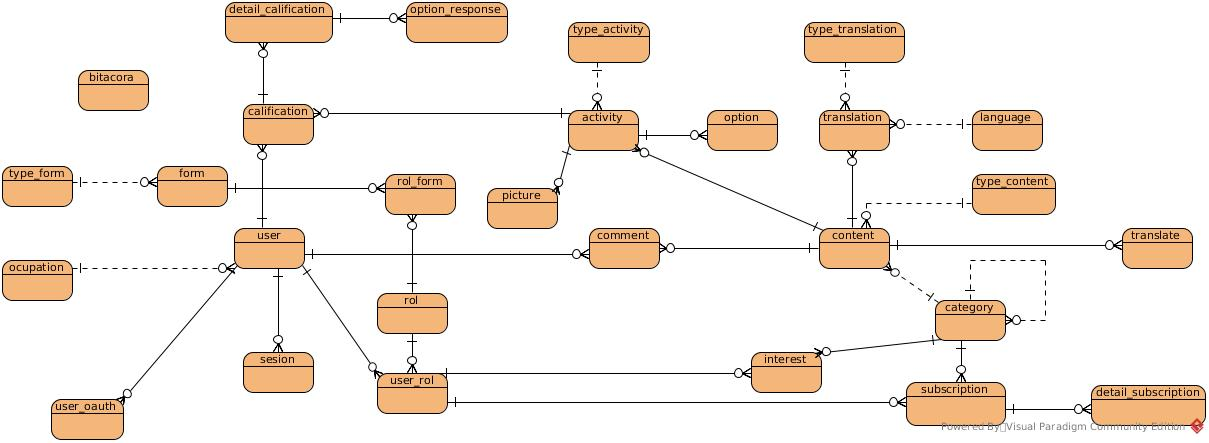
\includegraphics[angle=90, scale=0.4]{modelDatabase}
	\captionof{figure}{Modelo Base de Datos}
	\source{fuente: (Elaboración Propia)}
\end{minipage}
\newpage\cleardoublepage

\chapter{Documento de validación y aceptación 04-11-2014}

El presente documento tiene por finalidad el de constatar la conformidad tanto
del Cliente como el equipo de desarrollo.

Esta es la presentación de la versión alpha estipulado en la propuesta
técnica presentada Correspondiente al Sprint primero \textquotedblleft 
Versión Alpha listo\textquotedblright.

Dicha presentación está sujeto al pago del 17 (por ciento) del total del
costo del sistema, para Mayor conformidad para ambas partes se remarca los
siguientes aspectos.

\begin{enumerate}

\item \textbf{Escala de evaluación}

\begin{table}[!h]
\centering
\begin{tabular}{|c|c|c|}
\hline
\textbf{Punta je} & \textbf{Valor Numérico} & \textbf{Concepto} \\ \hline
NA & 0 & \begin{tabular}[c]{@{}c@{}}Se necesita hacer cambios\\ profundos\end{tabular} \\ \hline
RA & 1 & \begin{tabular}[c]{@{}c@{}}Requiere modificación para\\ aceptar\end{tabular} \\ \hline
A & 2 & Aceptado \\ \hline
\end{tabular}
\end{table}

\item \textbf{Las funcionalidades a presentar son las siguientes:}

\begin{itemize}

	\item Registro manual de usuario aprendiz a la plataforma.
		\begin{itemize}
			\item Envió de solicitud de confirmación de correo electrónico a bandeja de entrada.
			\item Modificar datos personales.
		\end{itemize}
	\item Registro por medio de red social.
		\begin{itemize}
			\item Registro por Facebook.
			\item Registro por Google.
			\item Registro por Twitter.
		\end{itemize}
	\item Implementar Página Maestra de Plataforma.

\end{itemize}

\item El pago del 17 (por ciento) se dará por hecho si se está conforme 
con 3 de las 4 funcionalidades.

\end{enumerate}

Se está conforme con una funcionalidad si se cumple los siguientes aspectos
estipulados en el sumario de evaluación de párrafos.

\section{Sumario de Evaluación de Parámetro}

\subsection{Registro manual de usuario aprendiz a la plataforma}

\textbf{Envió de solicitud de confirmación de correo electrónico a
bandeja de entrada}

Envió de solicitud de confirmación de correo electrónico a bandeja
de entrada. Abra un navegador web con la siguiente dirección (URL): plataforma
\footnote{plataforma: http:// plataformaeducativalael.hum.umss.edu.bo}, pinche en 
el enlace Registrar ubicado en la parte superior derecha.

\begin{table}[!htb]
\centering
\begin{tabular}{|l|l|l|}
\hline
\multicolumn{1}{|c|}{\textbf{N}} & \multicolumn{1}{c|}{\textbf{Parametros a evaluar}} & \multicolumn{1}{c|}{\textbf{Puntaje}} \\ \hline
01 & \begin{tabular}[c]{@{}l@{}}\textquestiondown Ud. puede ingresar datos en los campos y realizar clic en el botón\\ Registrar: Dirección de Correo, Nombre de Usuario, Contraseña, Repetir\\ Contraseña, Seleccione un valor de Ocupación, Sub Ocupación, Captcha?\end{tabular} &  \\ \hline
02 & \begin{tabular}[c]{@{}l@{}}\textquestiondown Ud. puede leer un mensaje \textquotedouble{Un correo electrónico que contiene m\'{a}s\\ instrucciones ha sido enviada bandeja de dirección de correo electrónico\\ proveedor}?\end{tabular} &  \\ \hline
03 & \begin{tabular}[c]{@{}l@{}}\textquestiondown Ud. ingrese a su cuenta de correo con la cual se registró anteriormente,\\ revise en bandeja spam, un mensaje de Administrador en el cuerpo un\\ enlace de confirmación?\end{tabular} &  \\ \hline
04 & \begin{tabular}[c]{@{}l@{}}\textquestiondown Ud. puede pinchar en el enlace y mostrarle el siguiente mensaje \textquotedouble{Su\\ dirección de correo electrónico ha sido verificado exitosa mente}, en la\\ parte superior de inicio sesión?\end{tabular} &  \\ \hline
\end{tabular}
\end{table}

Nota: Si está conforme con la funcionalidad \textquotedouble{Envió de
solicitud de confirmación de correo electrónico a bandeja de entrada}
si la sumatoria de Puntaje tiene un valor mayor y/o igual 5.

Las siguientes funcionalidades se realizan con credenciales propias.

\textbf{Modificar datos personales}

En la presentación principal en la parte superior derecha se tiene un enlace 
Inicio Sesión, pinchar sobre el mismo y mostrara una ventana de autentificar
con los siguientes campos: Nombre de Usuario, Contraseña.

\begin{table}[!htb]
\centering
\begin{tabular}{|l|l|l|}
\hline
\multicolumn{1}{|c|}{\textbf{N}} & \multicolumn{1}{c|}{\textbf{Parámetros a evaluar}} & \multicolumn{1}{c|}{\textbf{Puntaje}} \\ \hline
01 & \begin{tabular}[c]{@{}l@{}}\textquestiondown Ud. pude visualizar un Panel Administrativo en donde si tiene un mensaje\\ \textquotedouble{Hola} acompañado de su nombre de usuario en la parte superior derecha?\end{tabular} &  \\ \hline
02 & \begin{tabular}[c]{@{}l@{}}\textquestiondown Ud. puede visualizar un sus datos personales pinchando sobre la imagen\\ de una persona ubicada en la esquina superior derecha y presionar la\\ opción Perfil?\end{tabular} &  \\ \hline
03 & \begin{tabular}[c]{@{}l@{}}\textquestiondown Ud. puede editar sus datos personales pinchando en el enlace \textquotedouble{Actualizar\\ Usuario} ubicado en la parte inferior\end{tabular} &  \\ \hline
04 & \begin{tabular}[c]{@{}l@{}}\textquestiondown Ud. puede salvar sus datos pinchando en el bot\'{o}n \textquotedouble{Salvar} sobre el\\ c\'{o}digo verificación?\end{tabular} &  \\ \hline
05 & \begin{tabular}[c]{@{}l@{}}\textquestiondown Ud. puede cerrar sesión haciendo clic en la imagen del hombre cito\\ ubicado en la parte superior derecha del Panel Administrativo la opción\\ Cerrar Sesión?\end{tabular} &  \\ \hline
\end{tabular}
\end{table}

Nota: Si está conforme con la funcionalidad \textquotedouble{Modificar 
datos personales} si la sumatoria de Puntaje tiene un 
valor igual o mayor 6.

\section{Registro por medio de red social}

En la presentación principal en la parte superior derecha se tiene un enlace 
Inicio Sesión, pinchar sobre el mismo y mostrara una ventana de autentificar
con los siguientes enlaces:

\begin{itemize}
	\item Ingresar con Google.
	\item Ingresar con Facebook.
	\item Ingresar con Twitter.
\end{itemize}

Tomar en cuenta que para esta funcionalidad de registro por medio de red social
es con una cuenta de correo utilizada por primera vez en el sistema.

\begin{table}[!htb]
\centering
\begin{tabular}{|l|l|l|}
\hline
\multicolumn{1}{|c|}{\textbf{N}} & \multicolumn{1}{c|}{\textbf{Parametros a evaluar}} & \multicolumn{1}{c|}{\textbf{Puntaje}} \\ \hline
01 & \begin{tabular}[c]{@{}l@{}}\textquestiondown Ud. puede Registrarse pinchando sobre el bot\'{o}n Ingresar con Google\\ llenar con sus credenciales y un evento Login, le muestra un Panel\\ Administrativo donde en la parte superior derecha superior se muestra\\ su correo electrónico?\end{tabular} &  \\ \hline
02 & \begin{tabular}[c]{@{}l@{}}\textquestiondown Ud. puede cerrar sesión haciendo clic en la imagen del hombre cito\\ ubicado en la parte superior derecha del Panel Administrativo la opción\\ Cerrar Sesión?\end{tabular} &  \\ \hline
03 & \begin{tabular}[c]{@{}l@{}}\textquestiondown Ud. puede Registrarse pinchando sobre el bot\'{o}n Ingresar con Facebook\\ y llenando las credenciales de la red social y pinchando en el bot\'{o}n Login,\\ entonces le muestra un Panel Administrativo donde en la parte superior\\ derecha superior se muestra su correo electrónico?\end{tabular} &  \\ \hline
04 & \begin{tabular}[c]{@{}l@{}}\textquestiondown Ud. puede cerrar sesión haciendo clic en la imagen del hombre cito\\ ubicado en la parte superior derecha del Panel Administrativo la opción\\ Cerrar Sesión?\end{tabular} &  \\ \hline
05 & \begin{tabular}[c]{@{}l@{}}\textquestiondown Ud. puede Registrarse pinchando sobre el bot\'{o}n Ingresar con Twitter\\ llenar con sus credenciales y un evento Sign in luego dándole permiso de\\ autorización, le muestra un Panel Administrativo donde en la parte superior\\ derecha superior se muestra su correo electrónico?\end{tabular} &  \\ \hline
06 & \begin{tabular}[c]{@{}l@{}}\textquestiondown Ud. puede cerrar sesión haciendo clic en la imagen del hombre cito\\ ubicado en la parte superior derecha del Panel Administrativo la opción\\ Cerrar Sesión?\end{tabular} &  \\ \hline
\end{tabular}
\end{table}

Nota: Si está conforme con la funcionalidad \textquotedouble{Registro por 
medio de red social} si la sumatoria de Puntaje tiene un
valor mayor igual 6.

\section{Implementar página maestra de plataforma}

\begin{minipage}[!htb]{\hsize}\centering
\begin{tabular}{|l|l|l|}
\hline
\multicolumn{1}{|c|}{\textbf{N}} & \multicolumn{1}{c|}{\textbf{Parametros a evaluar}} & \multicolumn{1}{c|}{\textbf{Puntaje}} \\ \hline
01 & \begin{tabular}[c]{@{}l@{}}\textquestiondown Ud. puede reproducir un vídeo pinchando sobre la imagen \textquotedouble{VER\\ PRESENTACIÓN} ubicada en la parte superior de la Página Maestra?\end{tabular} &  \\ \hline
02 & \begin{tabular}[c]{@{}l@{}}\textquestiondown Ud. puede Registrarse pinchando sobre el bot\'{o}n Ingresar con Google\\ llenar con sus credenciales y un evento Login, le muestra un Panel\\ Administrativo donde en la parte inferior de Inicio, se muestra su correo\\ electrónico?\end{tabular} &  \\ \hline
\end{tabular}
\end{minipage}

Nota: Si está conforme con la funcionalidad \textquotedouble{Implementar 
Página Maestra de Plataforma} si la sumatoria de Puntaje tiene un valor 2.

Si se cumple el punto 3 procedemos a firmar este documento los representantes
para su aceptación.

\begin{minipage}[!htb]{\hsize}\centering
\begin{tabular}{|l|l|}
\hline
\begin{tabular}[c]{@{}l@{}}..........................................\\ Lic. Manuel Camacho Arce\\ PRODUCT OWNER\end{tabular} & \begin{tabular}[c]{@{}l@{}}.........................................\\ Juan Omar Huanca Balboa\\ SCRUM MASTER\end{tabular} \\ \hline
\end{tabular}
\end{minipage}\newpage\cleardoublepage

\chapter{Documento de validación y aceptación 26-01-2015}

El presente documento tiene por finalidad de constatar la conformidad tanto del
Cliente como el equipo de desarrollo.

Esta es la presentación de la versión Alpha estipulado en la propuesta 
técnica presentada Correspondiente al Sprint segundo, tercero \textquotedouble{
Versión Alpha listo}.

Dicha presentación está sujeto al pago del 4 (por ciento) del total del
costo del sistema, para Mayor conformidad para ambas partes se remarca los 
siguientes aspectos.

\begin{enumerate}

\item \textbf{Escala de evaluación}

\begin{table}[!h]
\centering
\begin{tabular}{|c|c|c|}
\hline
\textbf{Puntaje} & \textbf{Valor Numérico} & \textbf{Concepto} \\ \hline
NA & 0 & \begin{tabular}[c]{@{}c@{}}Se necesita hacer cambios\\ profundos\end{tabular} \\ \hline
RA & 1 & \begin{tabular}[c]{@{}c@{}}Requiere modificación para\\ aceptar\end{tabular} \\ \hline
A & 2 & Aceptado \\ \hline
\end{tabular}
\end{table}

\item \textbf{Las funcionalidades a presentar son las siguientes:}

\begin{itemize}

	\item Reiniciar Contraseña de Usuario (Usuario habilitado).
		\begin{itemize}
			\item Envió de solicitud de cambio de contraseña.
		\end{itemize}
	\item Gestión rol usuario Coordinador (Usuario habilitado).
	\item Gestionar Categoría (Usuario autentificado).
	\item Gestión rol usuario Tutor(Usuario habilitado, Sub categoría creada).
	\item Gestionar Contenido por intereses(Tener rol Tutor, Estar asignado a 
	sub categoría).
	\item Generar menú de tipos de contenido por Categoría(Contenido publicado).
		
\end{itemize}

\item \textbf{El pago del 4 (por ciento) se dar\'{a} por hecho si se está conforme 
con la mitad más uno de los puntos}

\end{enumerate}

Si está conforme con una funcionalidad si se cumple los siguientes aspectos
estipulados en el sumario de evaluación de párrafos.

\section{Sumario de Evaluación de parámetro}

\subsection{Reiniciar Contraseña de Usuario}

\textbf{Envió de solicitud de cambio de contraseña}

Requisito: Ser usuario habilitado, caso contrario utilizar las credenciales del
usuario por defecto; usuario: Juan Omar Huanca Balboa contraseña: autorregulado.

Abra un navegador web con la siguiente dirección (URL): plataforma 
\footnote{plataforma: http:// plataformaeducativalael.hum.umss.edu.bo} Pinche en
el enlace Iniciar Sesión ubicado en la parte superior derecha, seguido de
pinchar sobre en enlace Recuperar Contraseña.

\begin{minipage}[b]{\hsize}\centering
\begin{tabular}{|l|l|l|}
\hline
\multicolumn{1}{|c|}{\textbf{N}} & \multicolumn{1}{c|}{\textbf{Parametros a evaluar}} & \multicolumn{1}{c|}{\textbf{Puntaje}} \\ \hline
01 & \begin{tabular}[c]{@{}l@{}}Si Ud. eligió la cuenta por defecto llene, correo:\\ omar.huanca.balboa@gmail.com, contraseña:\\ omar.huanca.balboa. Captcha, pinchar sobre el bot\'{o}n Enviar\\ entonces ejecutar paso 03; caso contrario ingrese el correo\\ electrónico relacionado con la cuenta habilitada.\end{tabular} &  \\ \hline
02 & \begin{tabular}[c]{@{}l@{}}\textquestiondown Ud. puede ingresar datos en los campos: Dirección de Correo,\\ Captcha pinchar sobre el botón Enviar ?\end{tabular} &  \\ \hline
03 & \begin{tabular}[c]{@{}l@{}}\textquestiondown Ud. puede leer un mensaje \textquotedblleft Un correo electrónico que\\ contiene m\'{a}s instrucciones ha sido enviada bandeja de dirección\\ de correo electrónico asociada con su cuenta de proveedor\textquotedblright ?\end{tabular} &  \\ \hline
04 & \begin{tabular}[c]{@{}l@{}}\textquestiondown Ud. ingrese a su bandeja de mensajes del correo electrónico\\ ingresado anteriormente, un mensaje de Administrador -\\ Recuperar Contraseña en el cuerpo un enlace?\end{tabular} &  \\ \hline
05 & \begin{tabular}[c]{@{}l@{}}\textquestiondown Ud. pinche sobre el enlace le enviara a un formulario con los\\ siguientes campos: Contraseña, Repetir Contraseña?\end{tabular} &  \\ \hline
06 & \begin{tabular}[c]{@{}l@{}}\textquestiondown Ud. ingrese la nueva contraseña dos veces en los campos:\\ Contraseña, Repetir Contraseña y pinchar sobre el bot\'{o}n Enviar,\\ le muestra el siguiente mensaje \textquotedblleft Su dirección de correo ha sido\\ verificado\textquotedblright ?\end{tabular} &  \\ \hline
07 & \begin{tabular}[c]{@{}l@{}}\textquestiondown Si Ud. eligió la cuenta de usuario por defecto (autorregulado)\\ entonces ingrese la nueva contraseña pinche sobre el bot\'{o}n\\ Iniciar Sesión con sus nuevas credenciales caso contrario\\ ingrese la cuenta de usuario de la cuenta habilitada?\end{tabular} &  \\ \hline
\end{tabular}
\end{minipage}

Nota: Si está conforme con la funcionalidad \textquotedouble{Recobrar Contraseña} si la sumatoria
de Puntaje tiene un valor mayor y/o igual 4.

Las siguiente funcionalidad tiene que solicitar webmaster (administrador) que
agregue el rol coordinador en una cuenta habilitada, caso contrario puede hacer
uso de la cuenta por defecto nombre usuario: coordinador, contraseña: 
coordinador.

Ingrese la siguiente dirección URL en su navegador: plataforma 
\footnote{plataforma: http:// plataformaeducativalael.hum.umss.edu.bo}

Pinche en el enlace Iniciar Sesión ubicado en la parte superior derecha

\section{Gestión rol usuario Coordinador}

\begin{minipage}[b]{\hsize}\centering
\begin{tabular}{|l|l|l|}
\hline
\multicolumn{1}{|c|}{\textbf{N}} & \multicolumn{1}{c|}{\textbf{Parámetros a evaluar}} & \multicolumn{1}{c|}{\textbf{Puntaje}} \\ \hline
01 & \begin{tabular}[c]{@{}l@{}}\textquestiondown Si Ud. Eligió la cuenta habilitada tiene que dar a conocer al\\ webmaster a cual sub categor\'{i}a quiere estar asignado (Quechua \\ Básico, Quechua Psicosocial, Francés Básico, English Spread in \\ Cochabamba)? \\ \end{tabular} &  \\ \hline
02 & \begin{tabular}[c]{@{}l@{}}\textquestiondown Ud. Inicie sesión con las credenciales de la cuenta habilitada,\\ 
deber\'{i}a de aparecer nuevas opciones en el menú derecho de su \\ página principal de sesión?\end{tabular} &  \\ \hline
03 & \begin{tabular}[c]{@{}l@{}}\textquestiondown Ud. Puede solicitar al webmaster verbalmente que se pueden\\ revocar los privilegios asignados a la cuenta habilitada\\ mencionada anteriormente?\end{tabular} &  \\ \hline
\end{tabular}
\end{minipage}

Nota: Si está conforme con la funcionalidad \textquotedouble{Gestión 
rol usuario Coordinador} si la sumatoria de Puntaje tiene un
valor mayor y/o igual 2.

La siguiente funcionalidad tiene ingresar con una cuenta habilitada que tenga 
el rol de coordinador asignado correspondientemente. Caso contrario ingrese con
las credenciales Nombre Usuario: coordinador, Contraseña: coordinador.

Ingrese la siguiente dirección URL en su navegador: plataforma 
\footnote{plataforma: http:// plataformaeducativalael.hum.umss.edu.bo}
o pinche sobre la opción Inicio ubicado en el menú principal de la 
página de presentación Principal.

Pinche en el enlace Iniciar Sesión ubicado en la parte superior derecha.

\section{Gestionar Categoría}

\begin{minipage}[b]{\hsize}\centering
\begin{tabular}{|l|l|l|}
\hline
\multicolumn{1}{|c|}{\textbf{N}} & \multicolumn{1}{c|}{\textbf{Parámetros a evaluar}} & \multicolumn{1}{c|}{\textbf{Puntaje}} \\ \hline
01 & \begin{tabular}[c]{@{}l@{}}\textquestiondown Ud. Ingrese sus credenciales en los campos: Nombre Usuario,\\ Contraseña, le aparecer\'{a} una opción de su cuenta\\ administrativa?\end{tabular} &  \\ \hline
02 & \begin{tabular}[c]{@{}l@{}}\textquestiondown Ud. Pinche sobre la opción Categoría en la sub opción\\ Registrar Categoría y le muestra un formulario?\end{tabular} &  \\ \hline
03 & \begin{tabular}[c]{@{}l@{}}\textquestiondown Ud. Ingrese el nombre de la categoría padre con la categoría\\ 
reflexiva opción Padre, Archivo Respuesta Correcta, Archivo\\ Respuesta Incorrecta, pinchar sobre el bot\'{o}n Registrar, a\\
continuación deber\'{i}a mostrarle un detalle de la categoría padre\\ registrada?\end{tabular} &  \\ \hline
04 & \begin{tabular}[c]{@{}l@{}}\textquestiondown Ud. Pinche sobre la opción Categoría en la sub opción\\ Registrar Categoría y le muestra un formulario?\end{tabular} &  \\ \hline
05 & \begin{tabular}[c]{@{}l@{}}\textquestiondown Ud. Ingrese el nombre de la categoría hija con la categoría\\ reflexiva opción Hijo, Nivel Categoría, Imagen Categoría,\\ Descripción Categoría, Descripción Créditos, Descripción\\ Objetivos, pinchar sobre el botón Registrar, a continuación\\ debería mostrarle un detalle de la categoría hijo registrado?\end{tabular} &  \\ \hline
06 & \begin{tabular}[c]{@{}l@{}}\textquestiondown Ud. Pinche sobre la opción Categoría en la sub opción\\ Administrar Categoría y le muestra una tabla de categorias\\ registradas?\end{tabular} &  \\ \hline
07 & \begin{tabular}[c]{@{}l@{}}\textquestiondown Ud. elija una opción de la tabla, seguido podrá aplicar las\\ siguiente funcionalidades: Ver, Actualizar, Eliminar. Como\\ primera opción pinche sobre la opción Ver ubicado en la parte\\ derecha bajo la etiqueta Acción, podrá observar un detalle de los\\ campos con que cuenta la categoría?\end{tabular} &  \\ \hline
08 & \begin{tabular}[c]{@{}l@{}}\textquestiondown Ud. Pinche sobre la opción Categoría en la sub opción\\ Administrar Categoría y le muestra una tabla de categorías\\ registradas? \end{tabular} & \\ \hline
09 & \begin{tabular}[c]{@{}l@{}}\textquestiondown Ud. elija una opción de la tabla, como segunda opción pinche\\ sobre la acción Actualizar ubicado en la parte derecha bajo la\\ etiqueta Acción, podrá editar los campos previamente\\ registrados?\end{tabular} & \\ \hline
10 & \begin{tabular}[c]{@{}l@{}}\textquestiondown Ud. Pinche sobre la opción Categoría en la sub opción\\ Administrar Categoría y le muestra una tabla de categorías\\ registradas?\end{tabular} & \\ \hline
11 & \begin{tabular}[c]{@{}l@{}}\textquestiondown Ud elija una opción de la tabla, como tercera opción pinche\\ sobre la opción acción Borrar ubicado en la parte derecha bajo\\ la etiqueta Acción, un mensaje de confirmación le saldrá\\ pidiéndole aceptar o denegar?\end{tabular} & \\ \hline
12 & \begin{tabular}[c]{@{}l@{}}\textquestiondown Ud. Pinche sobre la opción Categoría en la sub opción\\ Administrar Categoría y le muestra una tabla de categorías\\ registradas?\end{tabular} & \\ \hline
13 & \begin{tabular}[c]{@{}l@{}}\textquestiondown Ud. Pinche sobre la opción Categoría en la sub opción Listar\\ Categoría y le muestra una lista de categorías registradas?\end{tabular} & \\ \hline
14 & \begin{tabular}[c]{@{}l@{}}\textquestiondown Ud. Podrá ordenar las categorías según el siguiente criterio:\\ Nombre Categoría, ubicado en la parte superior, inferior de la\\ lista?\end{tabular} & \\ \hline
\end{tabular}
\end{minipage}

Nota: Si está conforme con la funcionalidad \textquotedouble{Gestionar 
Categoría} si la sumatoria de Puntaje tiene un valor 
mayor y/o igual 7.

Las siguiente funcionalidad tiene que solicitar webmaster (administrador) que 
agregue el rol tutor en una cuenta habilitada, caso contrario puede hacer uso
de la cuenta por defecto nombre usuario: tutor, contraseña: tutor.

Ingrese la siguiente dirección URL en su navegador: plataforma 
\footnote{plataforma: http:// plataformaeducativalael.hum.umss.edu.bo} o pinche 
sobre la opción Inicio ubicado en el menú principal de la página 
de presentación Principal.

Pinche en el enlace Iniciar Sesión ubicado en la parte superior derecha.

\section{Gestión rol usuario Tutor}

\begin{minipage}[b]{\hsize}\centering
\begin{tabular}{|l|l|l|}
\hline
\multicolumn{1}{|c|}{\textbf{N}} & \multicolumn{1}{c|}{\textbf{Parámetros a evaluar}} & \multicolumn{1}{c|}{\textbf{Puntaje}} \\ \hline
01 & \begin{tabular}[c]{@{}l@{}}\textquestiondown Si Ud. Eligió la cuenta habilitada tiene que dar a conocer al\\ webmaster a cual sub categoría quiere estar asignado para poder\\  gestionar sus contenidos?\end{tabular} &  \\ \hline
02 & \begin{tabular}[c]{@{}l@{}}\textquestiondown Ud. Inicie sesión con las credenciales de la cuenta habilitada,\\ 
deber\'{i}a de aparecer las opciones en el menú derecho de su\\ página principal de sesión con los nombres: Mis Contenidos,\\ Actividad?\end{tabular} &  \\ \hline
03 & \begin{tabular}[c]{@{}l@{}}\textquestiondown Ud. Puede solicitar al webmaster verbalmente que se pueden\\ revocar los privilegios asignados a la cuenta habilitada\\ mencionada anteriormente?\end{tabular} &  \\ \hline
\end{tabular}
\end{minipage}

Nota: Si está conforme con la funcionalidad \textquotedouble{Gestión
rol usuario Tutor} si la sumatoria de Puntaje tiene un valor
mayor y/o igual 2.

Para realizar la siguiente funcionalidad, tiene que cumplir con la anterior
funcionalidad (Gestión rol usuario Tutor).

Ingrese la siguiente dirección URL en su navegador: plataforma 
\footnote{plataforma: http:// plataformaeducativalael.hum.umss.edu.bo} o pinche
sobre la opción Inicio ubicado en el menú principal de la página de 
presentación Principal.

Pinche en el enlace Iniciar Sesión ubicado en la parte superior derecha.

\section{Gestionar Contenido por intereses}

\begin{minipage}[b]{\hsize}\centering
\begin{tabular}{|l|l|l|}
\hline
\multicolumn{1}{|c|}{\textbf{N}} & \multicolumn{1}{c|}{\textbf{Parámetros a evaluar}} & \multicolumn{1}{c|}{\textbf{Puntaje}} \\ \hline
01 & \begin{tabular}[c]{@{}l@{}}\textquestiondown Ud. Ingrese sus credenciales en los campos: Nombre Usuario,\\ Contraseña, le aparecer\'{a} una opción de su cuenta\\ administrativa?\end{tabular} &  \\ \hline
02 & \begin{tabular}[c]{@{}l@{}}\textquestiondown Ud. Pinche sobre la opción Mis Contenidos a en la sub opción\\ Registrar Mi Contenido y le muestra un formulario?\end{tabular} &  \\ \hline
03 & \begin{tabular}[c]{@{}l@{}}\textquestiondown Ud. Ingrese el Título, Archivo Imagen, Seleccione el tipo de\\ contenido, Archivo Reproductor, Seleccione la sub categoría,\\ Fecha de liberación, Resumen, Archivo Resolución(*), Archivo\\ Glosario, Archivo Diccionario, Créditos pinchar sobre el botón\\ Registrar,a continuación debería mostrarle un detalle de la\\ categoría padre registrada?\end{tabular} &  \\ \hline
04 & \begin{tabular}[c]{@{}l@{}}\textquestiondown Ud. Pinche sobre la opci\'{o}n Mis Contenidos en la sub opción\\ Administrar Mis Contenidos y le muestra una tabla de\\ contenidos registradas?\end{tabular} &  \\ \hline
05 & \begin{tabular}[c]{@{}l@{}}\textquestiondown Ud. elija una opci\'{o}n de la tabla, como segunda opción pinche\\ sobre la acción Actualizar ubicado en la parte derecha bajo la\\ etiqueta Acción, podrá editar los campos previamente\\ registrados?\end{tabular} &  \\ \hline
06 & \begin{tabular}[c]{@{}l@{}}\textquestiondown Ud. Pinche sobre la opción Mis Contenidos en la sub opción\\ Administrar Mis Contenidos y le muestra una tabla de\\ contenidos registradas?\end{tabular} &  \\ \hline
07 & \begin{tabular}[c]{@{}l@{}}\textquestiondown Ud elija una opción de la tabla, como tercera opción pinche\\ sobre la opción acción Borrar ubicado en la parte derecha bajo\\ la etiqueta Acción, un mensaje de confirmación le saldrá\\ pidiéndole aceptar o denegar?\\\end{tabular} &  \\ \hline
08 & \begin{tabular}[c]{@{}l@{}}\textquestiondown Ud. Pinche sobre la opción Mis Contenidos en la sub opción\\ Listar Mis Contenidos y le muestra una lista de todos los\\ contenidos registrados? \end{tabular} & \\ \hline
09 & \begin{tabular}[c]{@{}l@{}}\textquestiondown Ud. Podra ordenar las categorías según el siguiente criterio:\\ Título, Fecha creación, Fecha liberación?\end{tabular} & \\ \hline
\end{tabular}
\end{minipage}

(*) Si usted define como tipo de contenido audio este campo es requerido.

Nota: Si está conforme con la funcionalidad \textquotedouble{Gestionar 
Contenido por intereses} si la sumatoria de Puntaje tiene un 
valor mayor y/o igual 5.

Ingrese la siguiente dirección URL en su navegador: plataforma 
\footnote{plataforma: http:// plataformaeducativalael.hum.umss.edu.bo} o pinche
sobre la opción Inicio ubicado en el men\'{u} principal de la página de 
presentación Principal o pinche sobre la opción Vista Página Principal
situado en la parte superior de su panel administrativo de su cuenta.

\section{Generar menú de tipos de contenido por Categoría}

\begin{minipage}[b]{\hsize}\centering
\begin{tabular}{|l|l|l|}
\hline
\multicolumn{1}{|c|}{\textbf{N}} & \multicolumn{1}{c|}{\textbf{Parámetros a evaluar}} & \multicolumn{1}{c|}{\textbf{Puntaje}} \\ \hline
01 & \begin{tabular}[c]{@{}l@{}}\textquestiondown Ud. Pinche sobre el tipo de categoría Audio/Vídeo si fuera el\\ caso con anterioridad, saldrá un elemento respecto la categoría\\  padre, pinche sobre el mismo y podrá ver una lista de sub\\ categorías asignadas al correspondiente idioma?\end{tabular} &  \\ \hline
02 & \begin{tabular}[c]{@{}l@{}}\textquestiondown Ud. Pinche sobre la imagen u/o nombre de la sub categoría ,\\
para poder ver contenido(s) creados relacionados con sub\\ categoría?\end{tabular} &  \\ \hline
03 & \begin{tabular}[c]{@{}l@{}}\textquestiondown Ud. Podrá ver una animación de desplazamiento de izquierda a\\ derecha de los contenidos comprendidos en la sub categoría, en\\ la parte inferior podrá ver los créditos y objetivos de todos los\\ episodios?\end{tabular} &  \\ \hline
\end{tabular}
\end{minipage}

Nota: Si está conforme con la funcionalidad \textquotedouble{Generar 
menú de tipos de contenido por Categoría} si la 
sumatoria de Puntaje tiene un valor mayor y/o igual 2.

Si se cumple más de los 4 puntos de 6 que fueron presentados a 
continuación procedemos a firmar este documento los representantes para su
aceptación.

\begin{minipage}[b]{\hsize}\centering
\begin{tabular}{|l|l|}
\hline
\begin{tabular}[c]{@{}l@{}}..........................................\\ Lic. Manuel Camacho Arce\\ PRODUCT OWNER\end{tabular} & \begin{tabular}[c]{@{}l@{}}.........................................\\ Juan Omar Huanca Balboa\\ SCRUM MASTER\end{tabular} \\ \hline
\end{tabular}
\end{minipage}
\newpage\cleardoublepage

\chapter{Licencia Pública General v.1} \label{chap:LPG-Bolivia}

\section{Introducción}

Según \cite{LPGBolivia} esta licencia está basada en la Licencia Pública
General GNU (GNU GPL) de la Fundación para el Software Libre (www.fsf.org),
la cual ha sida adaptada por la agencia para el Desarrollo de la Sociedad de
la Información en Bolivia (ADSIB) a la normativa legal vigente en Bolivia,
enmarcada en la Ley General de Telecomunicaciones, Tecnologías de la
Información y Comunicación, Ley 164 de 8 de agosto de 2011 y el Reglamento
por el Decreto Supremo 1793 de 13 de Noviembre de 2013.
 
\section{Preámbulo}

Según \cite{LPGBolivia} hablar de software libre, se refiere a la libertar
de acción, no de precio. La LPG-Bolivia esta diseñada para garantizar la.
libertad de distribuir copias de software libre (cobrar por ello si quiere).
Los desarrollado-res que usan la LPG-Bolivia protegen tus derechos con dos
pasos: 

\begin{itemize}

\item haciendo valer el derecho de propiedad intelectual en el software.

\item ofrece esta licencia que le da permiso legal para copiarlo,
distribuirlo y/o modificar-lo.
\end{itemize}

\section{Términos y Condiciones}

A continuación se referencia los beneficios de la licencia, para
mayor especificación revisar el documento: \cite{LPGBolivia}.

\subsection{Código Fuente}

Según \cite{LPGBolivia} el \textquotedouble{código fuente} de una obra es el
formato preferido de la misma para realizar modificaciones sobre ella.
\textquotedouble{Código Objeto} se refiere a cualquier formato de la obre que
no sea código fuente.

\subsection{Transmisión de Copias Legales}

Según \cite{LPGBolivia} se podrá cobrar cualquier importe o no cobrar nada por
cada copia que transmita y se podrá ofrecer soporte o protección de garantías
mediante un pago.


\end{document}
